\documentclass[12pt,a4paper]{article}
\usepackage[margin=1in]{geometry}
\usepackage{graphicx}
\usepackage{amsmath}
\usepackage{float}
\usepackage{caption}
\usepackage{subcaption}
\usepackage{booktabs}
\usepackage{hyperref}

\begin{document}

% Title Page
\begin{titlepage}
    \centering
    \vspace*{1.5cm}

    \Huge
    \textbf{Design of a CMOS OTA in BiCMOS8HP Technology}

    \vspace{2cm}

    \LARGE
    \textbf{Authors:}
    \vspace{0.5cm}\\
    Or Fachima  \\
    Arsen Arutyunov 

    \vspace{2cm}
    \large
    Date: 12/01/2025

    \vfill
\end{titlepage}

% Introduction
\section*{Introduction}
This report presents the design and simulation of a CMOS Operational Transconductance Amplifier (OTA) using the BiCMOS8HP technology. The primary objective is to achieve a high-performance OTA that meets specific requirements for gain, bandwidth, phase margin, and power efficiency. The design process involves careful selection of components, circuit optimization, and detailed simulation to ensure compliance with the desired specifications. Through this work, various aspects of analog circuit design are explored, including stability analysis, noise performance, and transient behavior.

% Circuit Design and Schematic
\section*{Circuit Design and Schematic}
\subsection*{Device Parameters}
The table below summarizes the key parameters for the transistors and other components used in the design:

\begin{table}[H]
    \centering
    \begin{tabular}{@{}lccccc@{}}
    \toprule
    \textbf{Device} & \textbf{Length (L)} & \textbf{Width (W)} & \textbf{$g_m$ (uS)} & \textbf{$g_{ds}$ (uS)} \\
    \midrule
    M1 & 0.4$\mu$m & 12$\mu$m & 910.2 & 14.48 \\
    M2 & 0.4$\mu$m & 12$\mu$m & 910.2 & 14.48 \\
    M3 & 3.6$\mu$m & 120$\mu$m & 437.4 & 7.555 \\
    M4 & 3.6$\mu$m & 120$\mu$m & 437.4 & 7.555 \\
    M5 & 0.7$\mu$m & 2.8$\mu$m & 531.3 & 28.35 \\
    M6 & 0.2$\mu$m & 28.8$\mu$m & 1542 & 32.17 \\
    M7 & 3.1$\mu$m & 10.2$\mu$m & 605.5 & 21.02 \\
    M8 & 0.7$\mu$m & 0.3$\mu$m & 52.13 & 3.612 \\
    \midrule
    Cc & \multicolumn{4}{c}{1.1pF} \\
    R0 & \multicolumn{4}{c}{147.1k$\Omega$} \\
    R3 & \multicolumn{4}{c}{7k$\Omega$} \\
    \bottomrule
    \end{tabular}
    \caption{Summary of device parameters in the OTA design.}
    \label{tab:parameters}
\end{table}
\pagebreak
\subsection*{Schematics}
The following figures illustrate the OTA schematics with operating currents and voltages:

\begin{figure}[H]
    \centering
    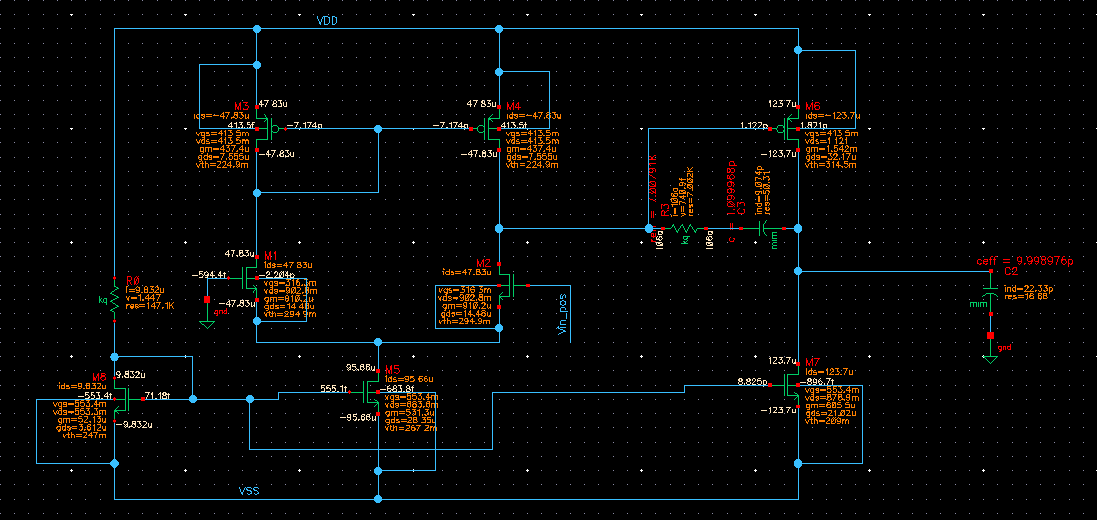
\includegraphics[width=0.8\textwidth]{scematic_OTA.png}
    \caption{OTA schematic with currents.}
    \label{fig:ota_currents}
\end{figure}

\begin{figure}[H]
    \centering
    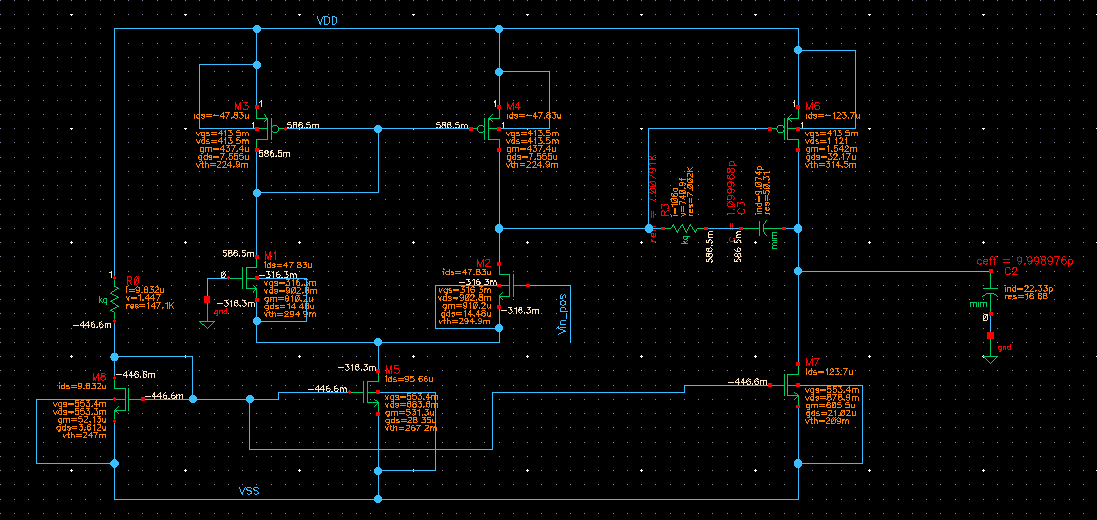
\includegraphics[width=0.8\textwidth]{scematic_OTA_DC.png}
    \caption{OTA schematic with operating voltages.}
    \label{fig:ota_voltages}
\end{figure}
\pagebreak

% Simulation Results
\section*{Simulation Results}



\subsection*{DC Analysis}
\subsubsection*{Power Calculation}
The power consumption was analyzed based on the voltage and current sources. The calculation is shown below:
\begin{equation*}
    P = V \cdot I = 2 \cdot 229.2\mu = 458.4\mu \text{Watt}
\end{equation*}
\begin{figure}[H]
    \centering
    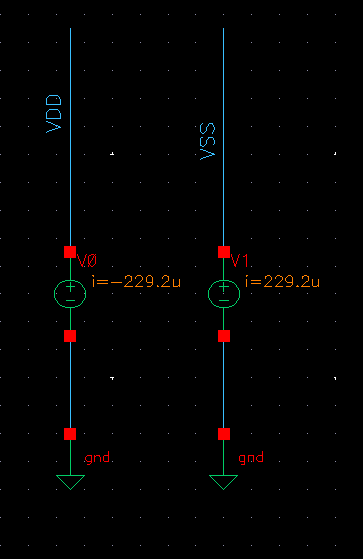
\includegraphics[width=0.6\textwidth]{DC_power.png}
    \caption{Power calculation based on DC voltage and current sources.}
    \label{fig:dc_power}
\end{figure}
\pagebreak
\subsection*{AC Analysis}
\subsubsection*{Frequency and Phase Response}
The gain and phase response are shown in the same plot. The achieved gain is 61.49 dB with a bandwidth of 90.6 kHz. The unity gain frequency was 50.46 MHz, and the phase at this frequency (from the AC simulation) is -130 degrees.

It is important to note that the unity gain frequency is lower than the GBW. This behavior arises because the system is not a purely single-pole system. While it was possible to achieve a perfect separation of poles, we opted for a trade-off to reduce power consumption.
 The gain-bandwidth product (GBW) was calculated as follows:
\begin{equation*}
    \text{GBW} = \text{Gain} \cdot \text{BW} = 10^{\frac{61.49}{20}} \cdot 90.6\text{kHz} = 107.55\text{MHz}
\end{equation*}
\begin{figure}[H]
    \centering
    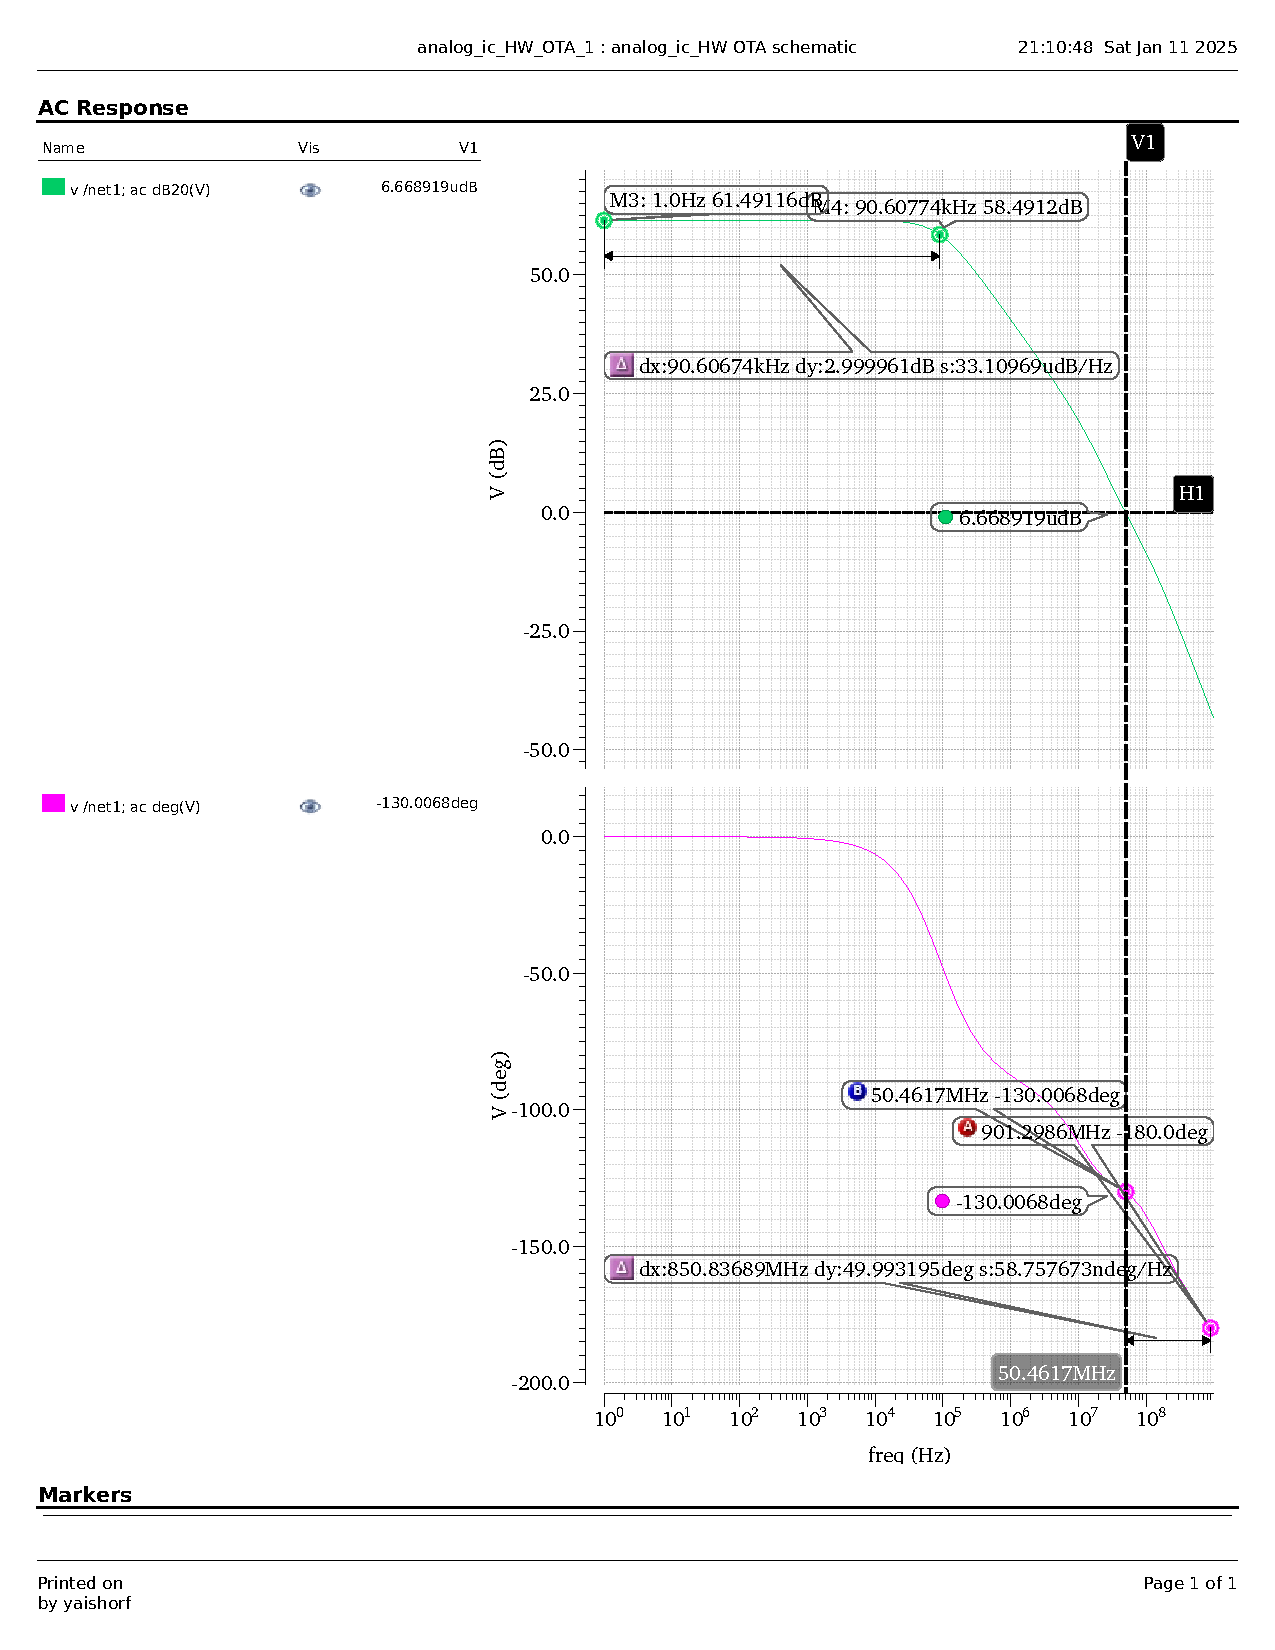
\includegraphics[width=0.8\textwidth]{ac_results.pdf}
    \caption{AC simulation results showing gain and phase response.}
    \label{fig:ac_results}
\end{figure}
\pagebreak
\subsubsection*{CMRR Results}
To efficiently compute the CMRR, a test bench was created to calculate both the differential and common-mode gains. The test bench is shown in the figure below:

\begin{figure}[H]
    \centering
    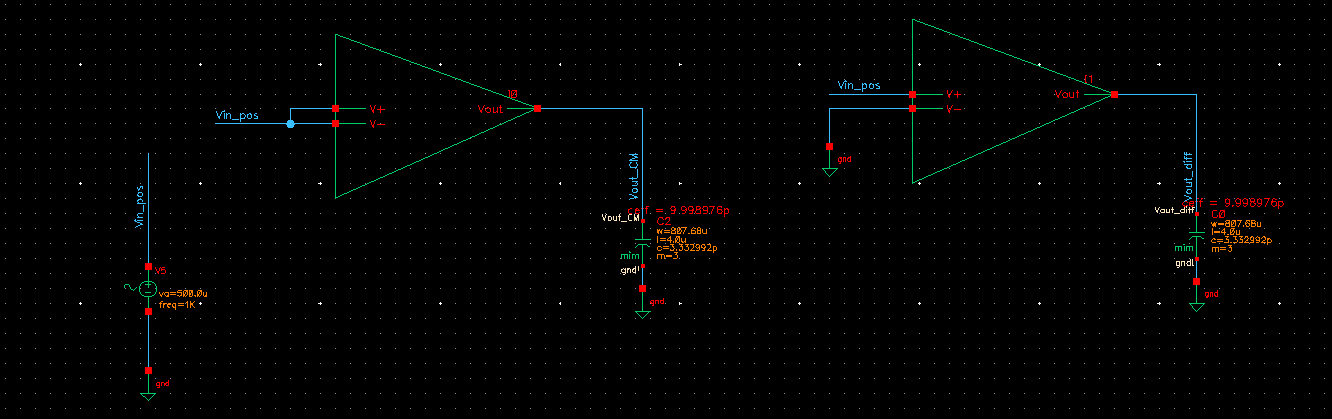
\includegraphics[width=0.8\textwidth]{OTA_t.png}
    \caption{Test bench for calculating differential and common-mode gains.}
    \label{fig:ota_test_bench}
\end{figure}

The CMRR was calculated using the formula:
\begin{equation*}
    \text{CMRR} = 20 \cdot \log_{10}\left(\frac{A_{\text{diff}}}{A_{\text{cm}}}\right)
\end{equation*}
\begin{figure}[H]
    \centering
    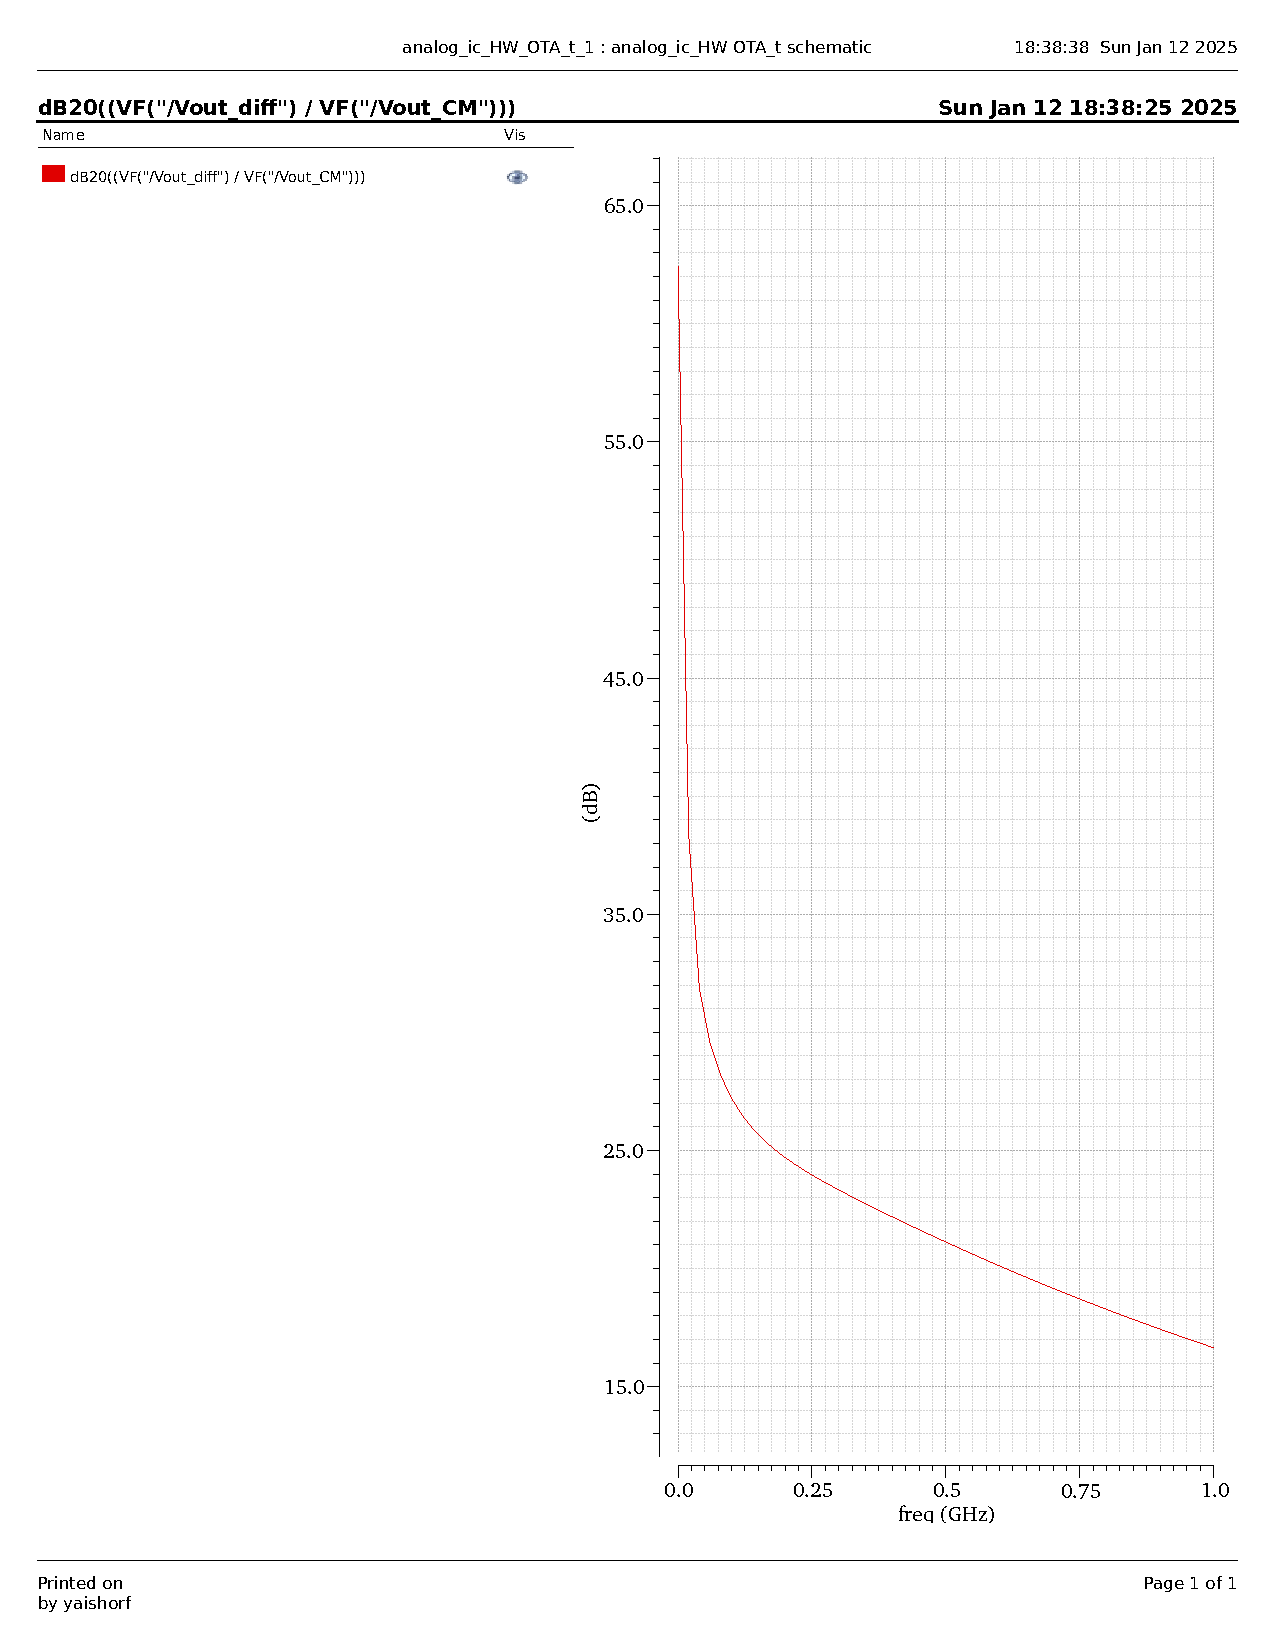
\includegraphics[width=0.8\textwidth]{CMRR.pdf}
    \caption{CMRR results showing the calculated values.}
    \label{fig:cmrr}
\end{figure}
The following figure shows a comparison of the common-mode and differential gains:
\begin{figure}[H]
    \centering
    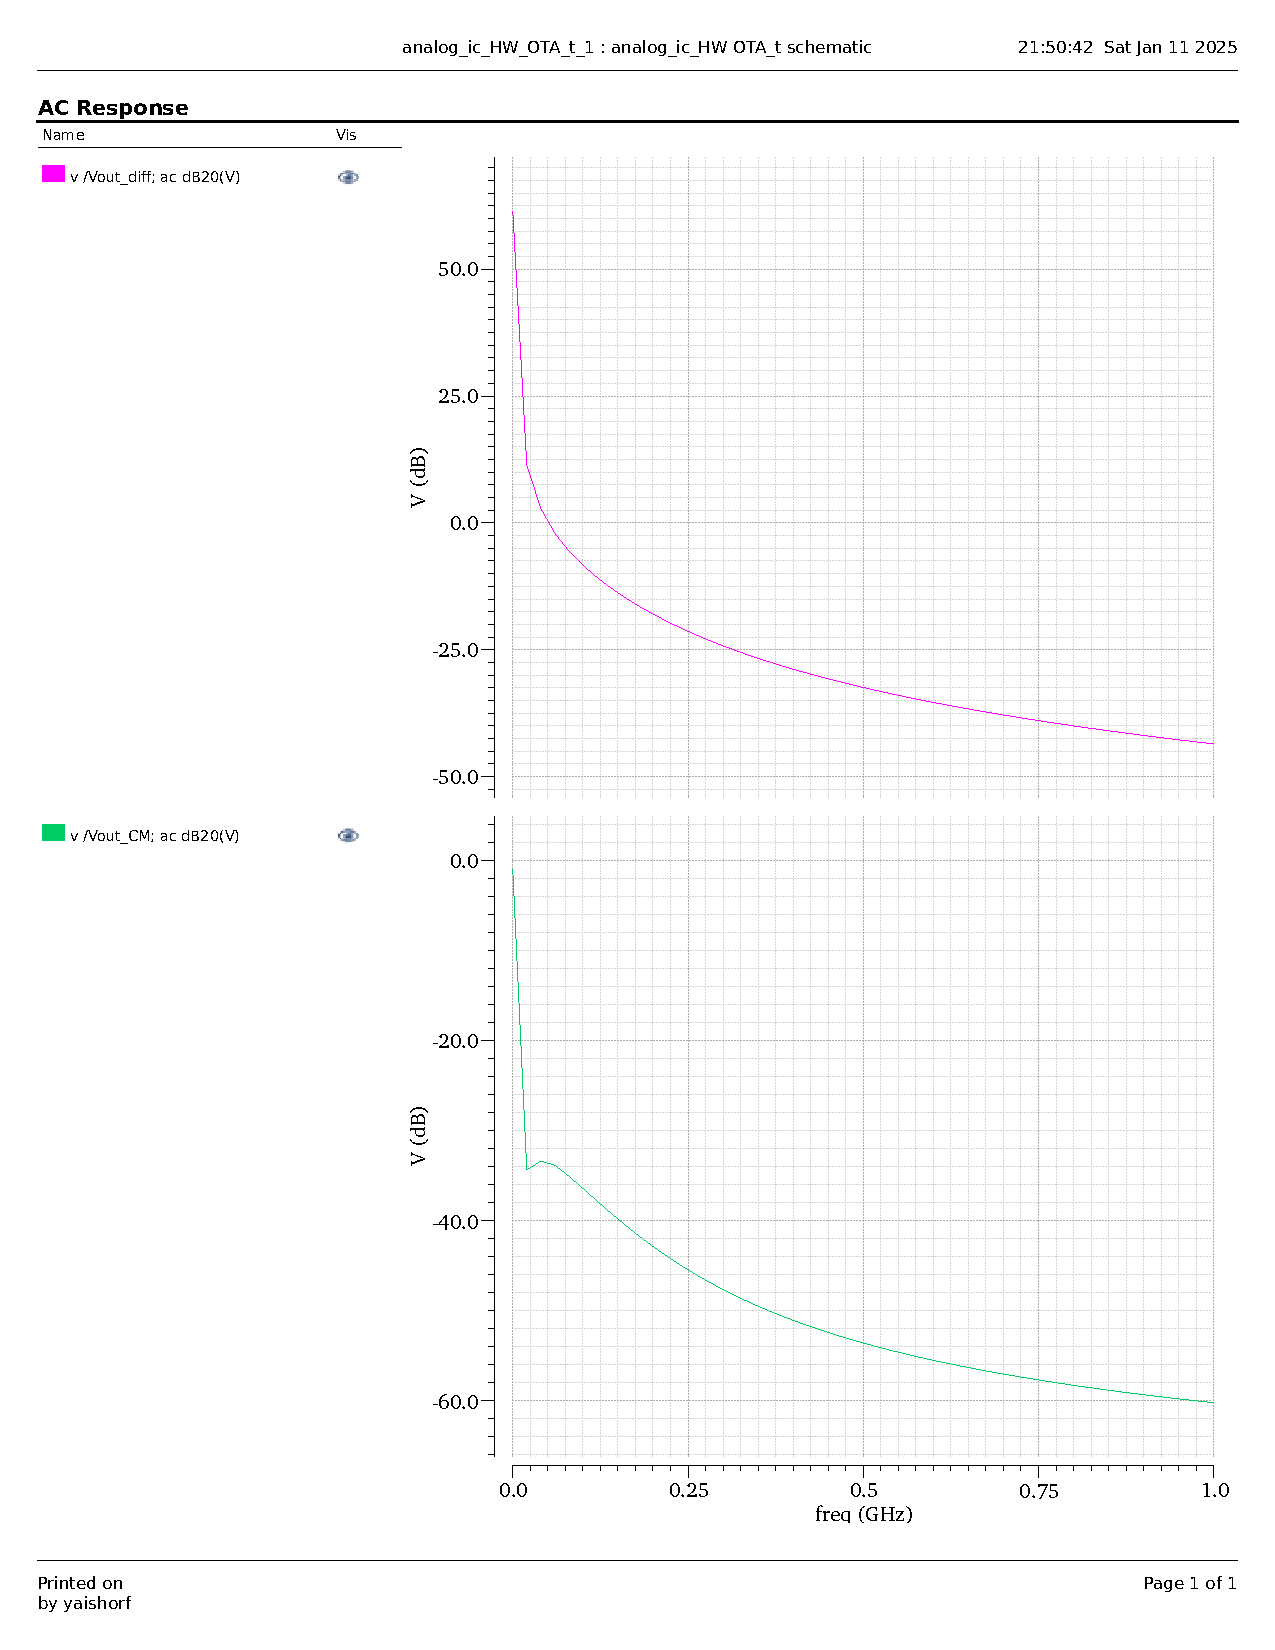
\includegraphics[width=0.8\textwidth]{cm_vs_diff.pdf}
    \caption{Common-mode versus differential gain plots.}
    \label{fig:cm_vs_diff}
\end{figure}
It is evident that the circuit rejects the common-mode signal efficiently and predominantly amplifies the differential signal.
\pagebreak
\subsubsection*{Input and Output Impedance}
The input and output impedance of the circuit were analyzed using the results shown in the following figures:
\begin{figure}[H]
    \centering
    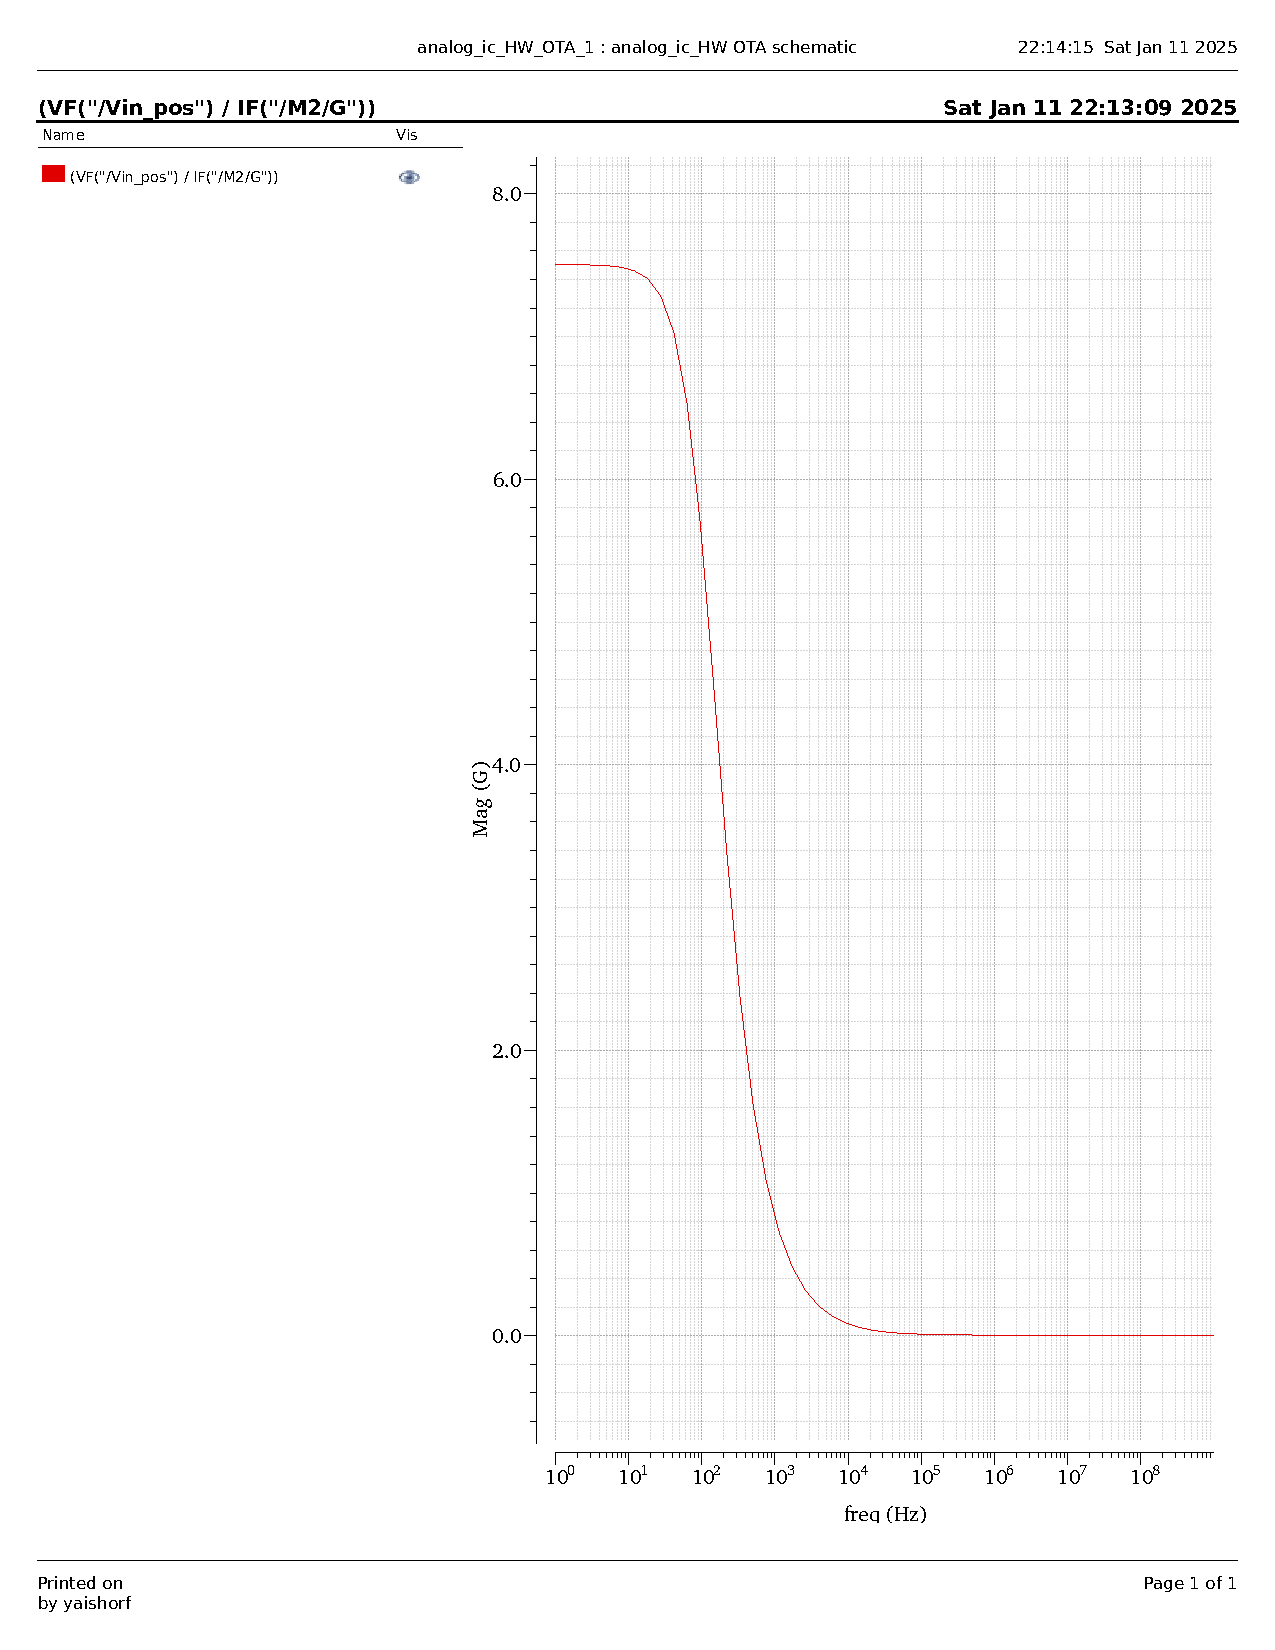
\includegraphics[width=0.8\textwidth]{in_impednce.pdf}
    \caption{Input impedance analysis showing a high value of approximately 8G$\Omega$ for low frequencies, typical for OTA gate input.}
    \label{fig:input_impedance}
\end{figure}

\begin{figure}[H]
    \centering
    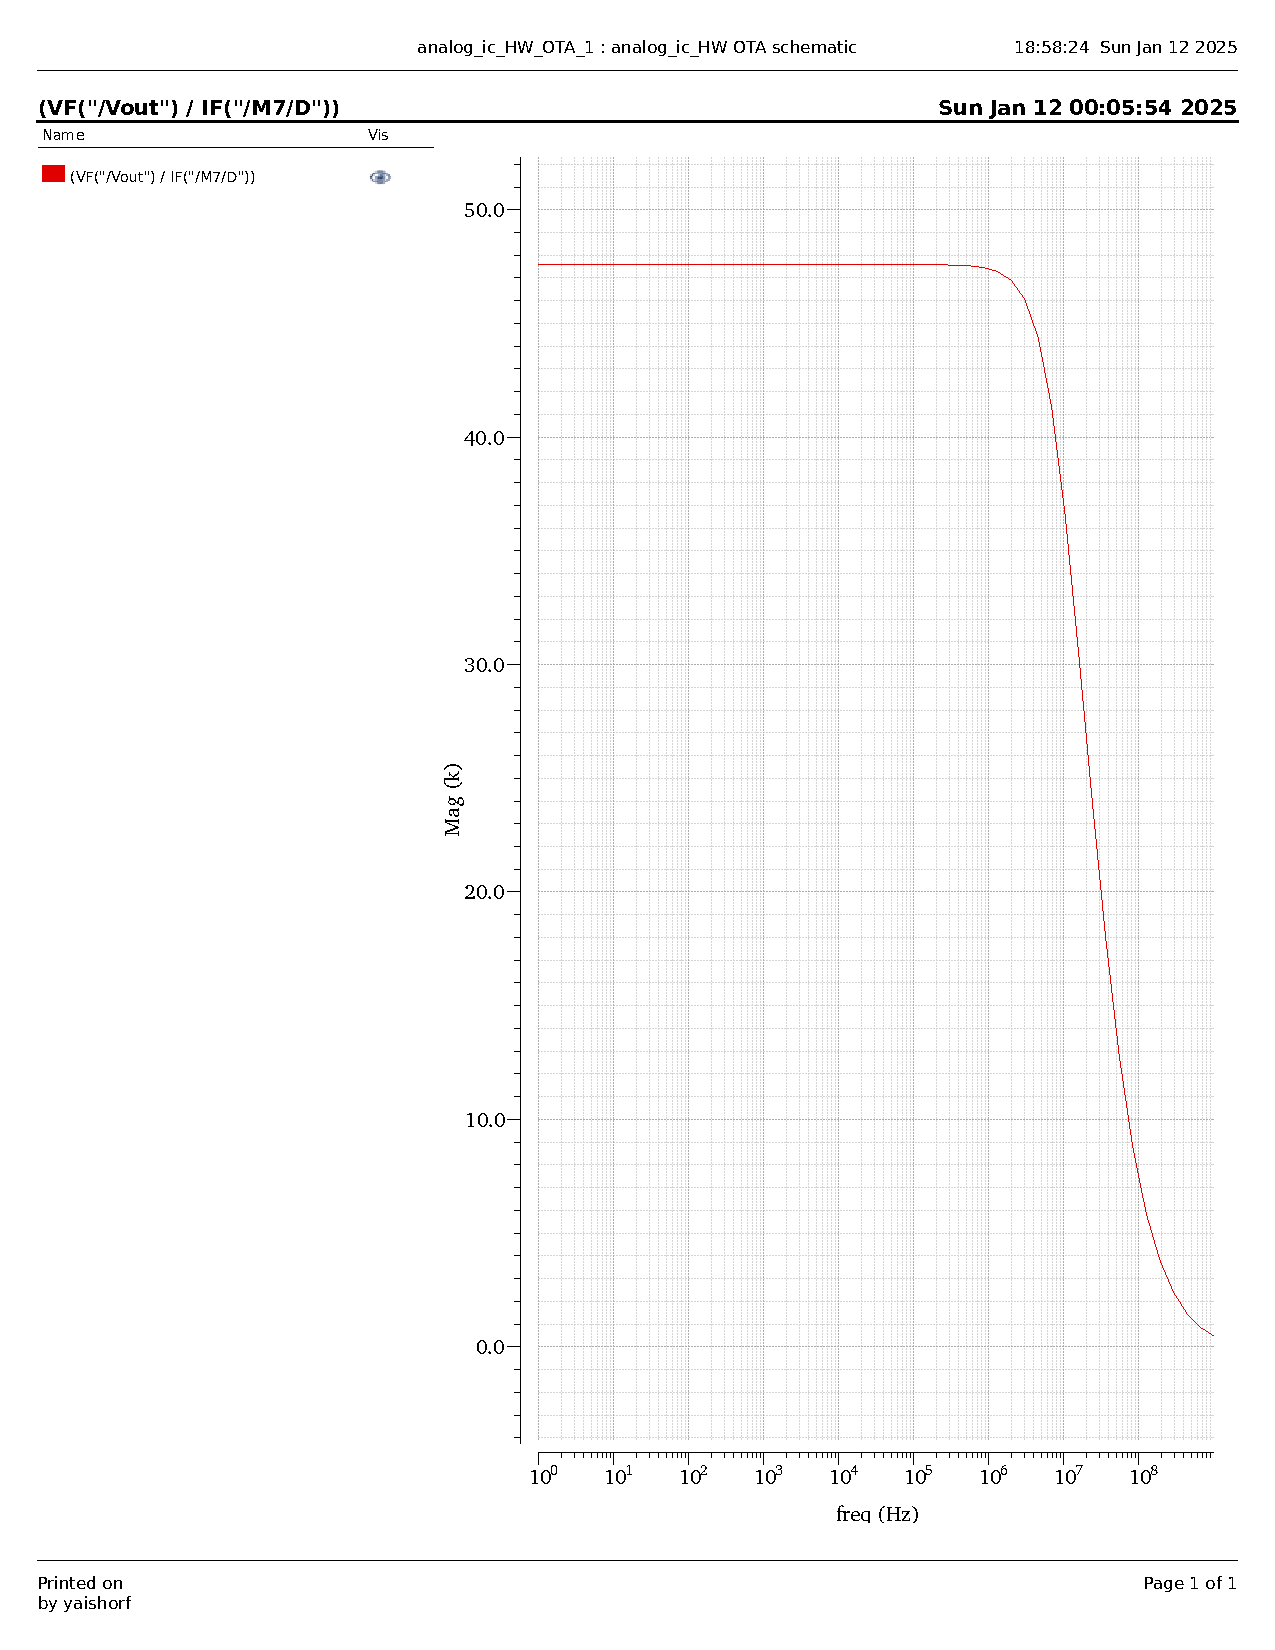
\includegraphics[width=0.8\textwidth]{Rout.pdf}
    \caption{Output impedance analysis showing a value of approximately 47.5k$\Omega$.}
    \label{fig:output_impedance}
\end{figure}
\pagebreak
\subsection*{Transient Analysis}

For the transient analysis, a sinusoidal input signal with an amplitude of 0.5 mV and a frequency of 1 kHz was applied. The output signal was observed to be symmetric with an approximate amplitude of 540 mV. A slight asymmetry of 4 mV was noted. The following figures show the output signal and its zero-centered version for clarity:

\begin{figure}[H]
    \centering
    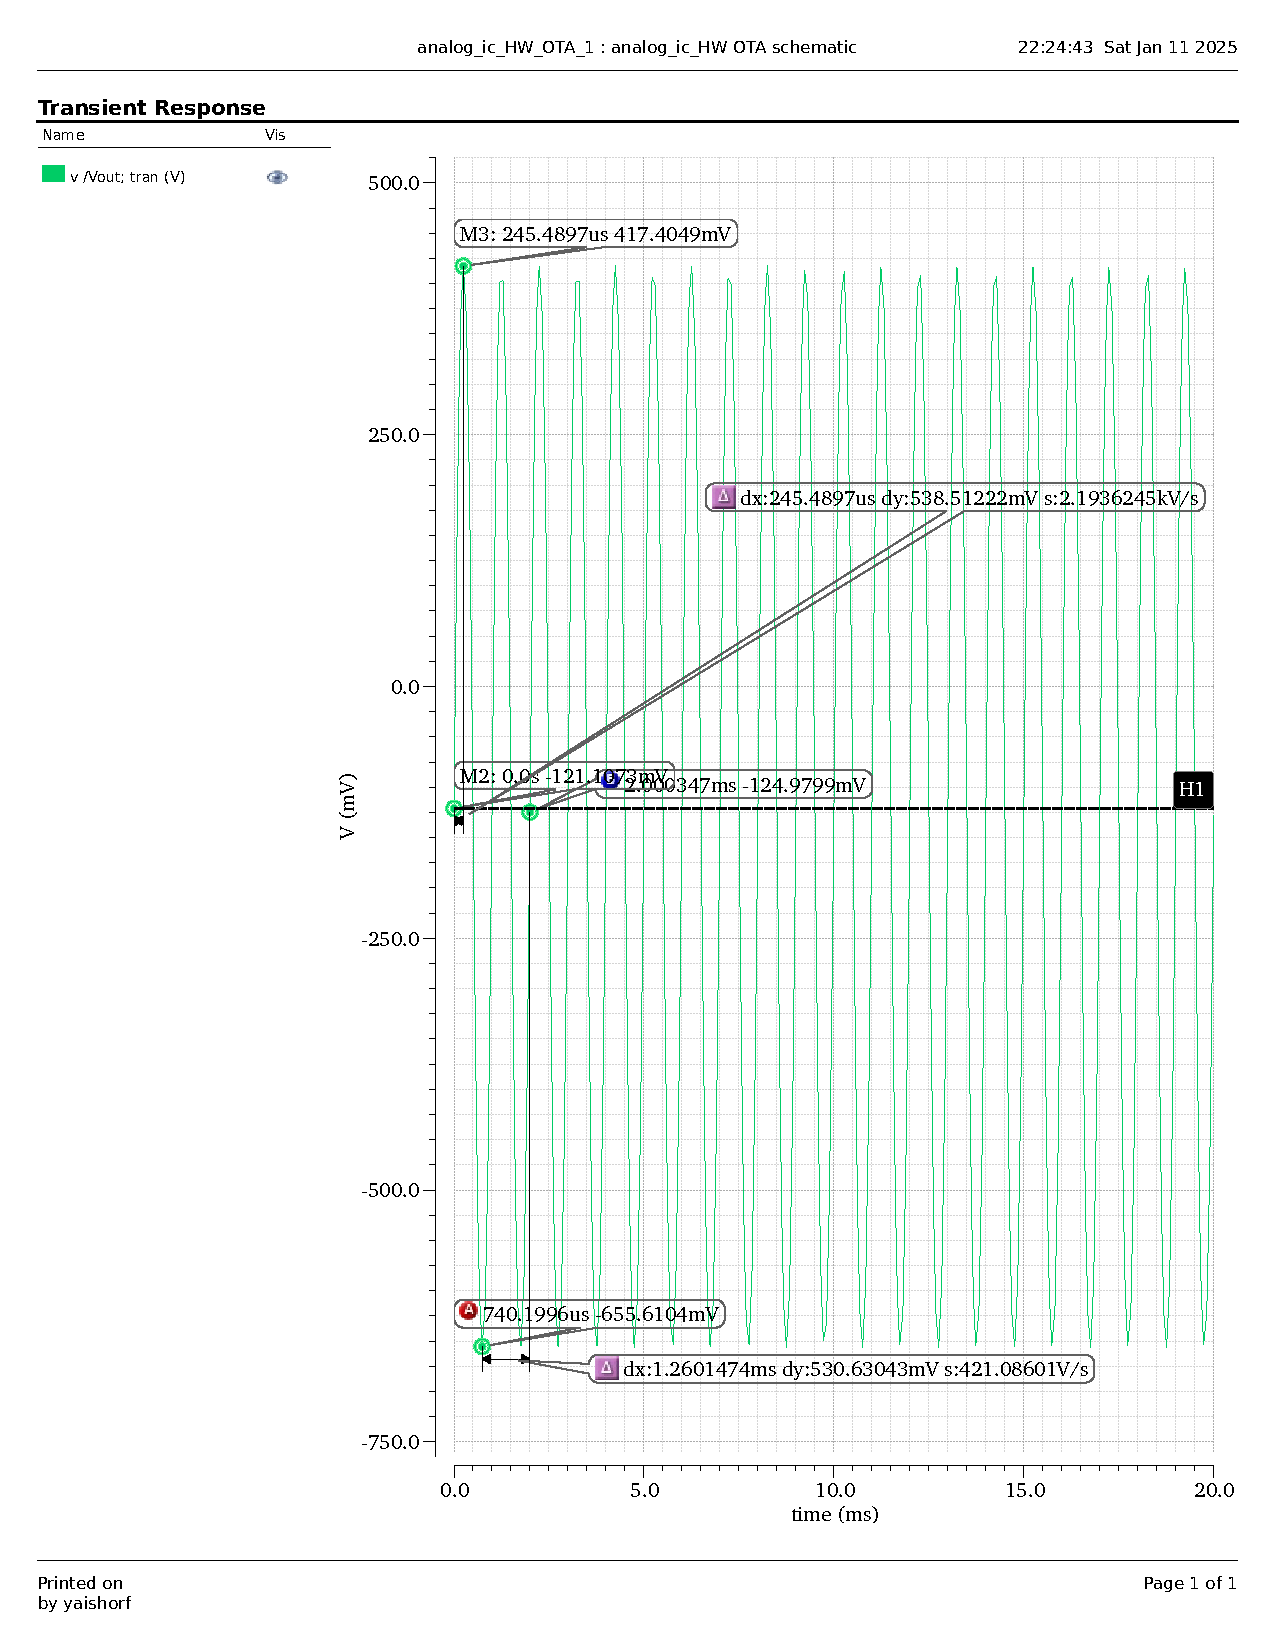
\includegraphics[width=0.8\textwidth]{tran.pdf}
    \caption{Output signal for a sinusoidal input of 0.5 mV amplitude at 1 kHz.}
    \label{fig:tran}
\end{figure}

\begin{figure}[H]
    \centering
    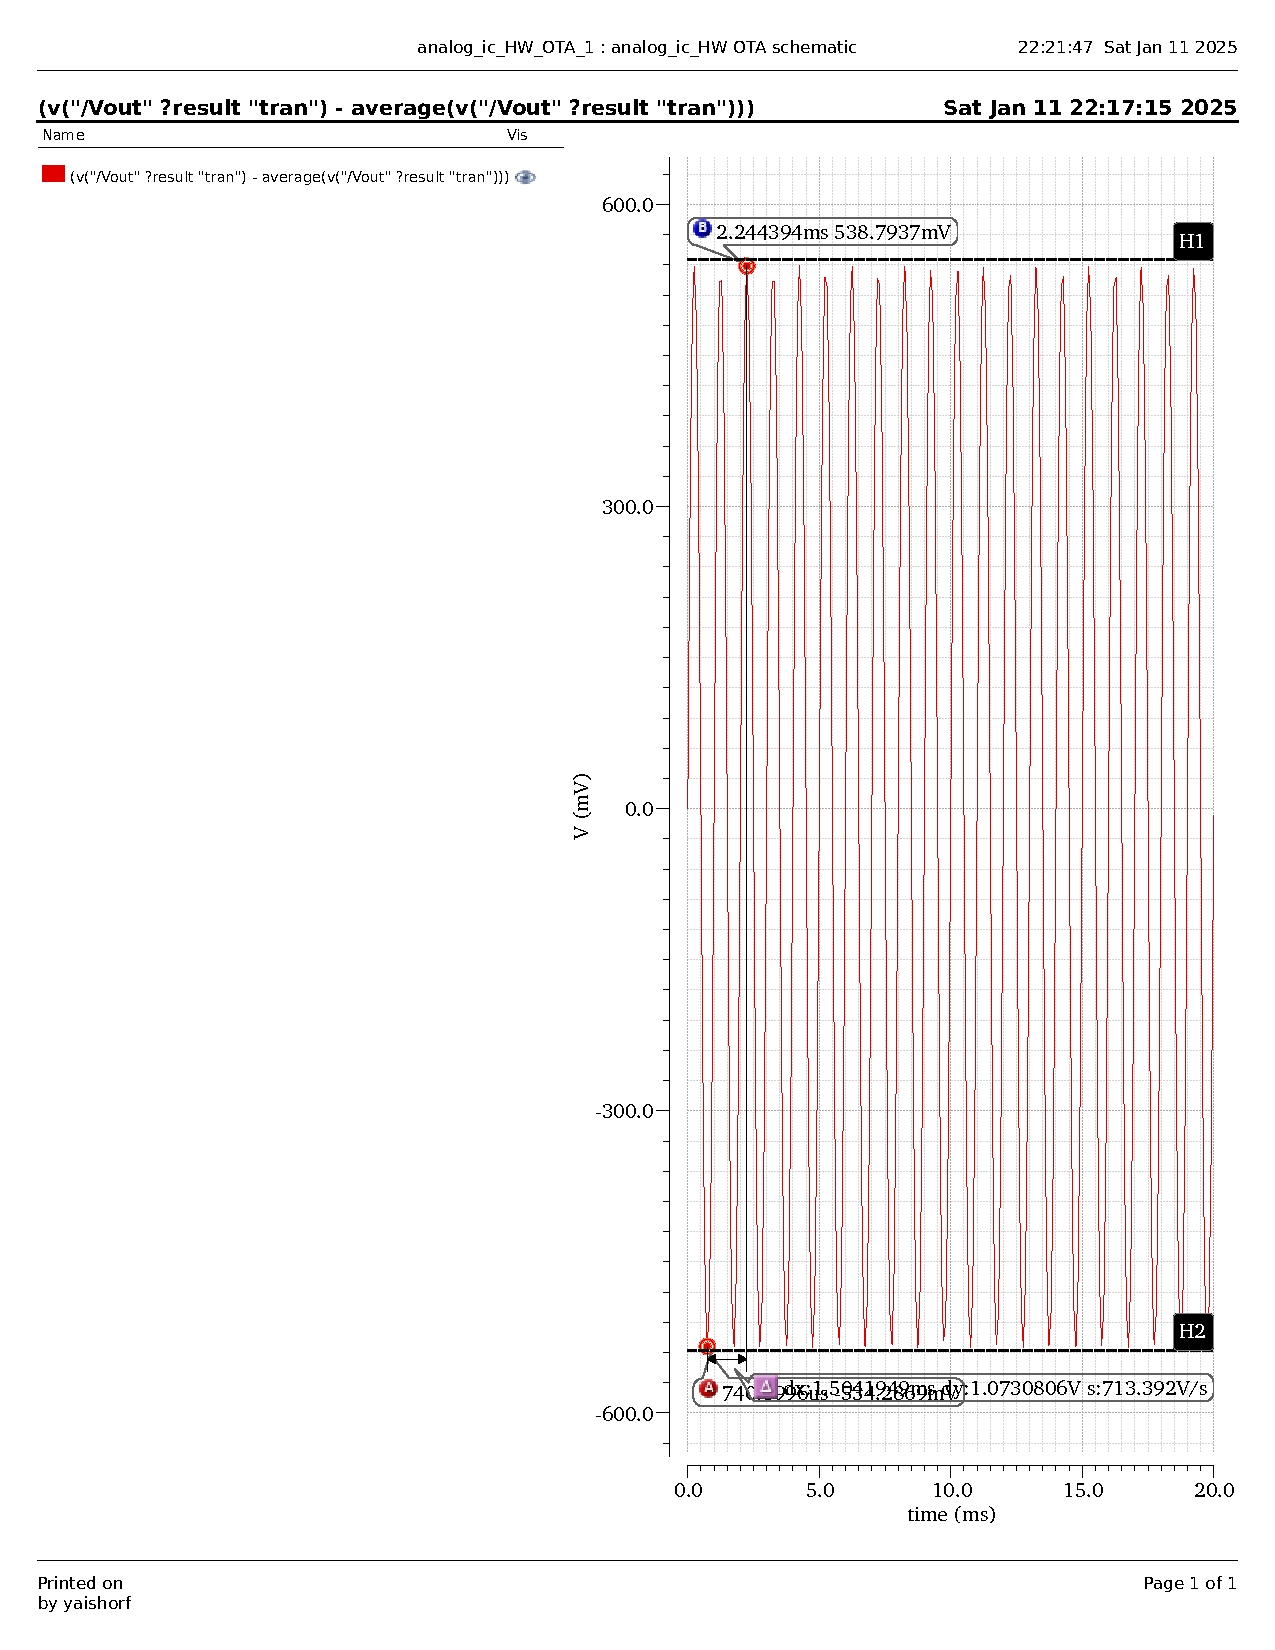
\includegraphics[width=0.8\textwidth]{tran1.pdf}
    \caption{Zero-centered version of the output signal for better visualization.}
    \label{fig:tran1}
\end{figure}
\newpage
\subsubsection*{Slew Rate (SR)}

To measure the SR, a pulse signal with an amplitude of 1 V was applied to evaluate the speed at the output. Using the simulator's calculator, the measured value was:

\[
\text{SR} = 81 \, \text{V/µs}.
\]

This was also measured analytically by calculating the derivative of $V_{\text{out}}$ over time. The analytical result aligns well with the theoretical relationship:

\[
\text{Slew Rate} = \frac{I_5}{C_c} = \frac{95\, \mu \text{A}}{1.1\, \text{pF}} \approx 86.3 \, \text{V/µs}.
\]

The following figures illustrate the results from both methods:

\begin{figure}[H]
    \centering
    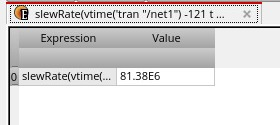
\includegraphics[width=0.8\textwidth]{SR3.jpg}
    \caption{Slew rate measurement using the simulator's calculator.}
    \label{fig:SR3}
\end{figure}
This was also measured analytically by calculating the derivative of Vout over time.
\begin{figure}[H]
    \centering
    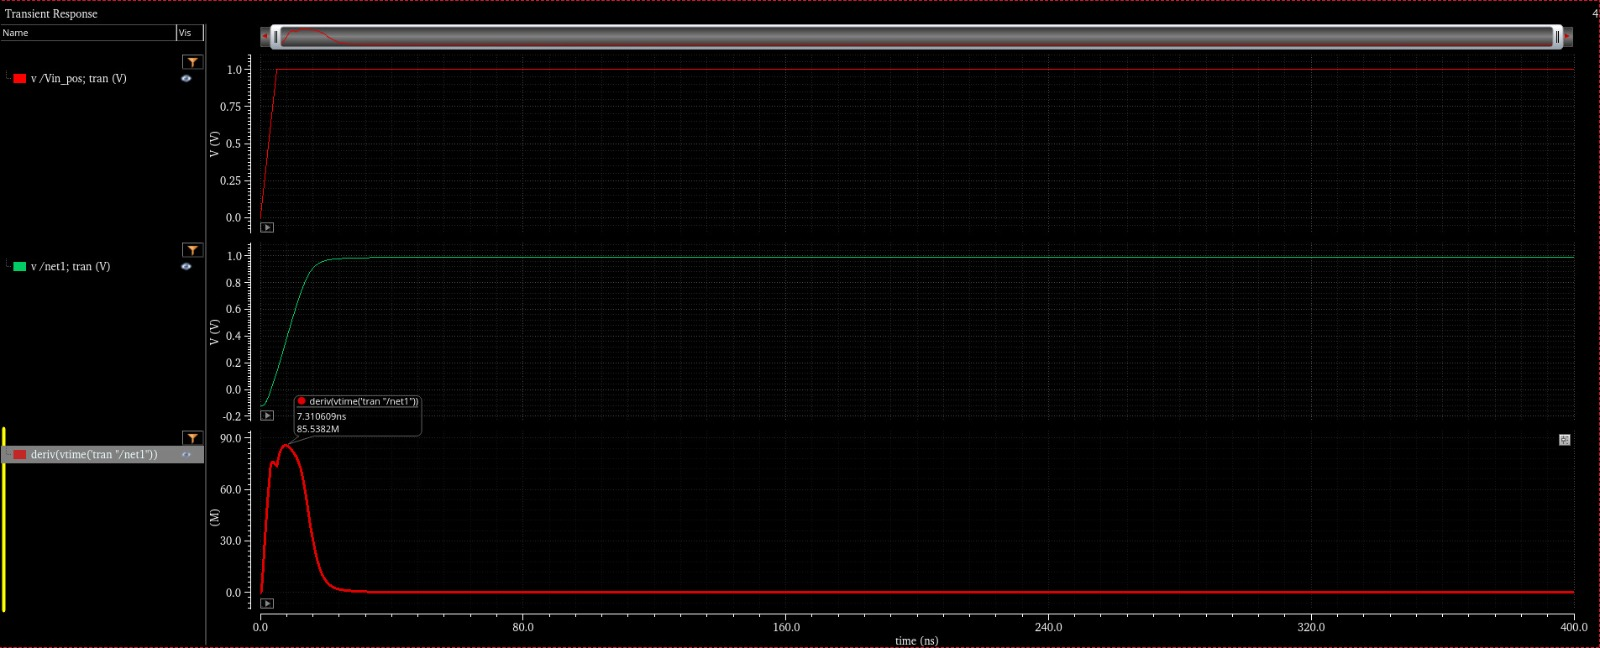
\includegraphics[width=0.8\textwidth]{SR2.jpg}
    \caption{Measurement of the slew rate based on the derivative of $V_{\text{out}}$ over time.}
    \label{fig:SR2}
\end{figure}

\pagebreak

\subsection*{Noise Analysis}
The noise analysis was conducted to evaluate the output voltage and current noise. It can be observed that the output voltage noise increases approximately by the gain (about 1000) relative to the input voltage noise. This behavior is expected and aligns with the amplifier's gain characteristics.

Additionally, the total integrated noise over the bandwidth was calculated using the simulator's calculator with the integration limits set to match the bandwidth. The integrated noise is shown in the figure below:

\begin{figure}[H]
    \centering
    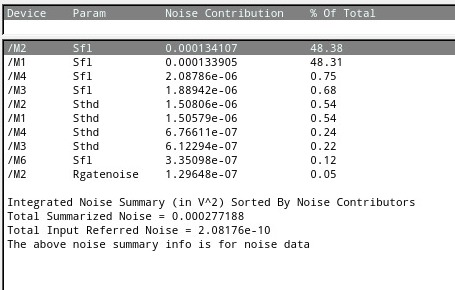
\includegraphics[width=0.8\textwidth]{noise_integ.jpg}
    \caption{Total integrated noise over the bandwidth.}
    \label{fig:noise_integ}
\end{figure}

\begin{figure}[H]
    \centering
    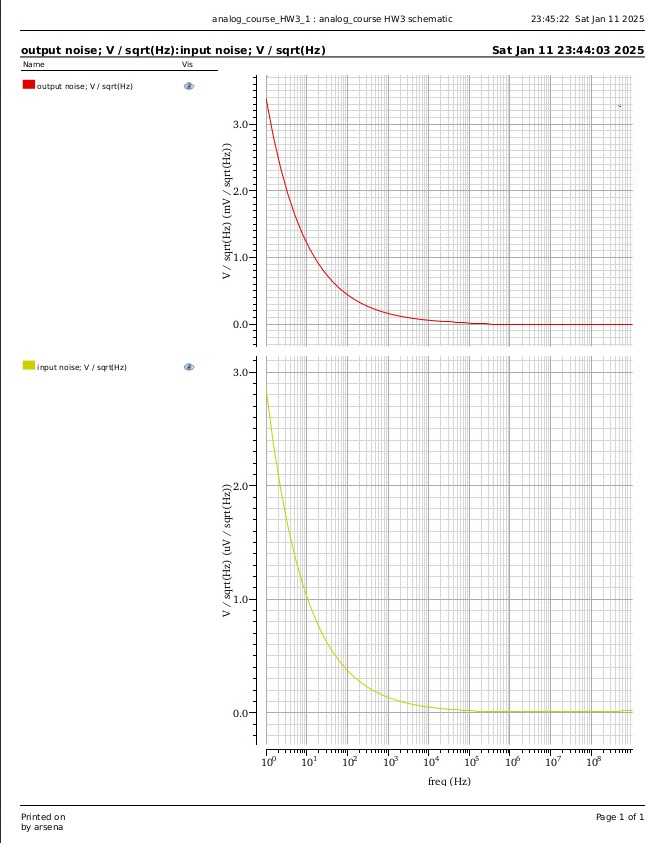
\includegraphics[width=0.8\textwidth]{V_noise.jpg}
    \caption{Output voltage noise simulation result.}
    \label{fig:voltage_noise}
\end{figure}

\begin{figure}[H]
    \centering
    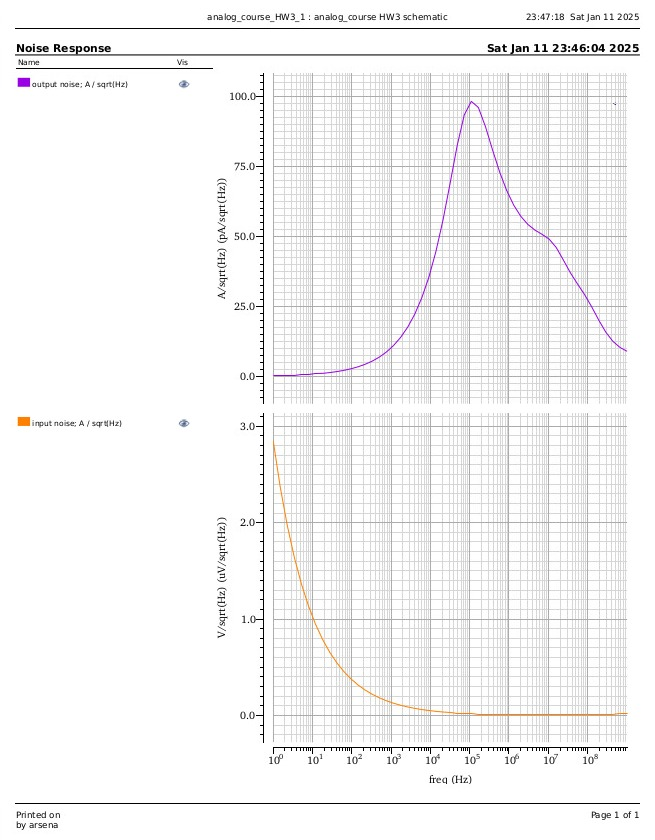
\includegraphics[width=0.8\textwidth]{I_noise.jpg}
    \caption{Output current noise simulation results.}
    \label{fig:current_noise}
\end{figure}
\newpage
Additionally, the top 10 noise contributors at 100MHz were analyzed and summarized in the following figure:

\begin{figure}[H]
    \centering
    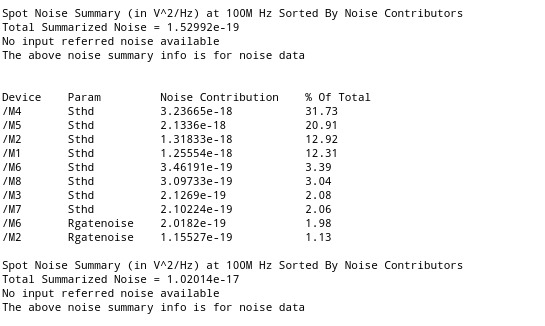
\includegraphics[width=0.8\textwidth]{noise_summary.jpg}
    \caption{Top 10 noise contributors in the OTA design.}
    \label{fig:noise_summary}
\end{figure}

It is noteworthy that M4 ranks as the highest contributor to the noise, which aligns with its size and role in the circuit. Interestingly, M3, despite having the same size as M4, contributes significantly less noise, highlighting differences in their operational conditions and roles in the circuit.

\pagebreak

\subsection*{Stability Analysis}
To achieve accurate results, a stability simulation was performed. The results were as follows:
\begin{itemize}
    \item Gain Margin (GM): 46 dB
    \item Phase Margin (PM): 49.07 degrees 
\end{itemize}

The following figure illustrates the stability plot from the simulation:

\begin{figure}[H]
    \centering
    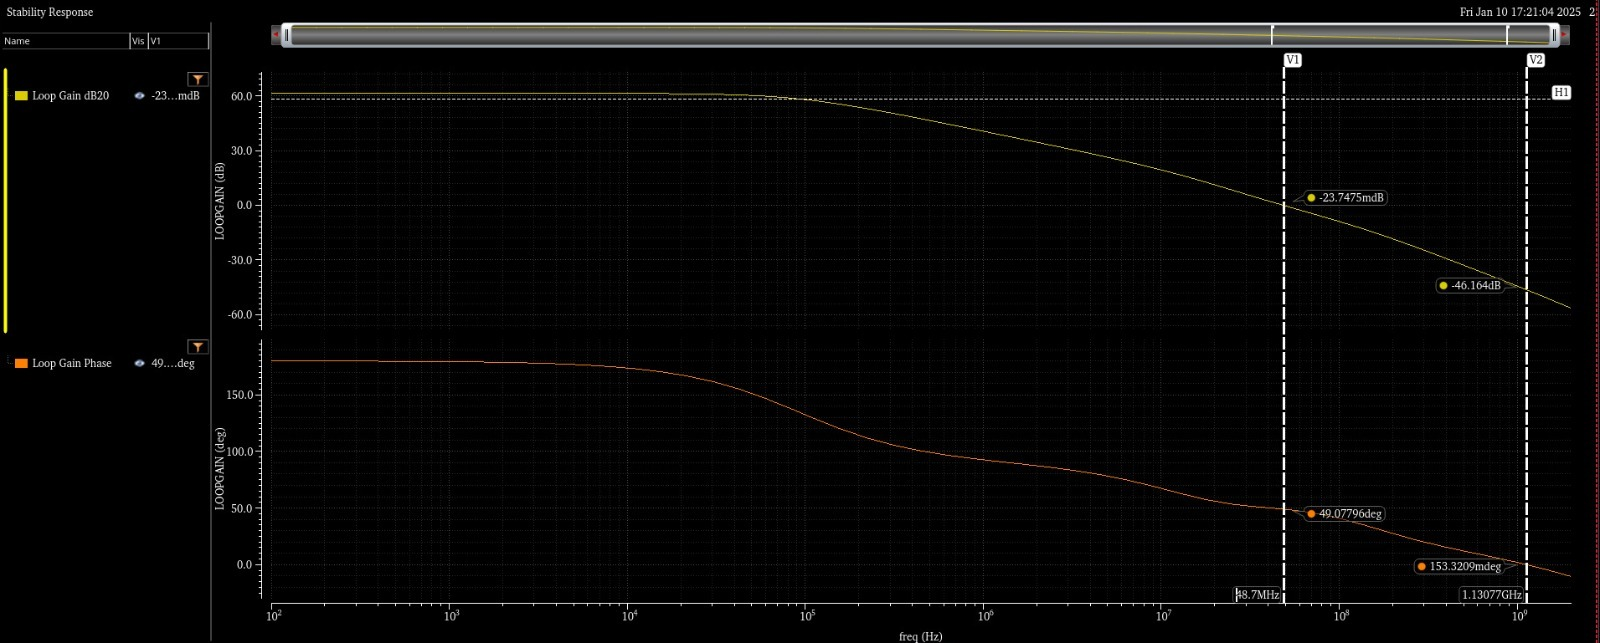
\includegraphics[width=0.8\textwidth]{stability.jpg}
    \caption{Stability simulation results showing gain and phase margins.}
    \label{fig:stability}
\end{figure}
\pagebreak

\section*{Discussion and Observations}
When we started the task, we initially followed the equations strictly to achieve the desired ratios. This approach led to excessively large transistor sizes and significant current consumption. The turning point in the task came when we decided to focus on the principles rather than the exact numerical results. This shift allowed us to design a circuit that, in our opinion, is far more optimal compared to the initial design.

We will now summarize the steps and considerations taken during the design process, categorized by the components involved:

\textbf{M8:}  
M8 was designed to provide a stable bias voltage for the current mirrors and the input stage. Its sizing was optimized to  minimize its impact on the overall power consumption.

\textbf{M5:}  
M5 serves as the current source for the first stage. While it is not the sole factor affecting $g_{m1}$, it plays a significant role in limiting its values. Furthermore, M5 strongly impacts the gain of the first stage due to the reduction of $R_{out4}$ as the current increases. The sizing of M5 was adjusted to balance the trade-off between gain and current consumption. See Figure~\ref{fig:gm1_w5}.  

\textbf{M1 and M2:}  
To achieve the desired $g_{m1}$ for a GBW greater than 100 MHz, we carefully sized M1 and M2. We initially determined the current through these transistors and then adjusted their lengths and widths to achieve a $g_{m1}$ of approximately 3.14 m. This value, along with a compensation capacitor of half the load capacitance ($C_c = 0.5C_L$), enabled us to reach the GBW target. However, to reduce parasitic capacitances, we opted for a $g_{m1}$ value reduced by a factor of 3 and compensated for it with a smaller $C_c$. Finally, as the gain was slightly below the desired level, we fine-tuned the widths of M1 and M2 to minimize $V_{ov}$, ensuring the required gain. See Figure~\ref{fig:gm1_w1}.


\textbf{M3 and M4:}  
To ensure proper gain in the second stage while maintaining reasonable transistor sizes, we adjusted the lengths and widths of M3 and M4. A key consideration was reducing the $V_{ov}$ of M6 by slightly decreasing the length of M4. This optimization ensured the required $V_{ov}$ for M6 in order to increase the gain . See Figures~\ref{fig:G2_W4}.

\textbf{M6 and M7:}  
Initially, M6 and M7 were sized very large to ensure the desired pole splitting and phase margin. However, this resulted in high power consumption and excessive transistor sizes. To optimize this stage, we introduced a compensation resistor ($R_3$) and fine-tuned the compensation capacitor ($C_c$), which allowed us to reduce the sizes of M6 and M7 significantly while maintaining a PM above 45 degrees. Additionally, the channel length of M7 was increased to improve the output resistance and ensure the desired gain. Finally, $W_6$ was adjusted to achieve a symmetric output swing.

\textbf{Compensation Capacitor and Resistor:}  
The compensation components were critical for optimizing the GBW and PM. Initially, we set $C_c$ to half the load capacitance and $R_3$ to zero. This setup resulted in a low GBW and high PM. By carefully tuning $C_c$ and $R_3$, we observed a significant improvement in GBW, which increased from below 100 MHz to 110 MHz, and a stable PM above 45 degrees. Furthermore, the optimized $C_c$ and $R_3$ reduced the influence of the zero introduced by $R_3$, allowing for smaller $g_m$ values in M6 and M7, thereby reducing power consumption. See Figures~\ref{fig:GBW_Cc} and \ref{fig:GBW_R3}.

This systematic optimization process allowed us to achieve the desired specifications while minimizing power consumption and maintaining performance within the required parameters.

\section*{Summary of Achieved Results}

The table below summarizes the required specifications and the achieved results for the CMOS OTA design. The measured output swing was found to be \( -0.884 \, \text{V} \) to \( 0.884 \, \text{V} \), as illustrated in Figure~\ref{fig:swing}. 

\begin{table}[H]
    \centering
    \begin{tabular}{@{}lcc@{}}
        \toprule
        \textbf{Parameter}       & \textbf{Required} & \textbf{Achieved}       \\ 
        \midrule
        Gain ($A_0$)             & 60 dB             & 61.49 dB               \\ 
        Gain Bandwidth (GBW)     & 100 MHz           & 107.5 MHz              \\ 
        Phase Margin (PM)        & >45°              & 49°                    \\ 
        Unity Gain Frequency     & Not specified     & 50.4 MHz               \\ 
        Power Consumption        & Not specified     & 458 µW                 \\ 
        Dynamic Range            & Not specified     & -0.884 V to 0.884 V    \\ 
        \bottomrule
    \end{tabular}
    \caption{Summary of required specifications and achieved results.}
    \label{tab:summary_results}
\end{table}

\begin{figure}[H]
    \centering
    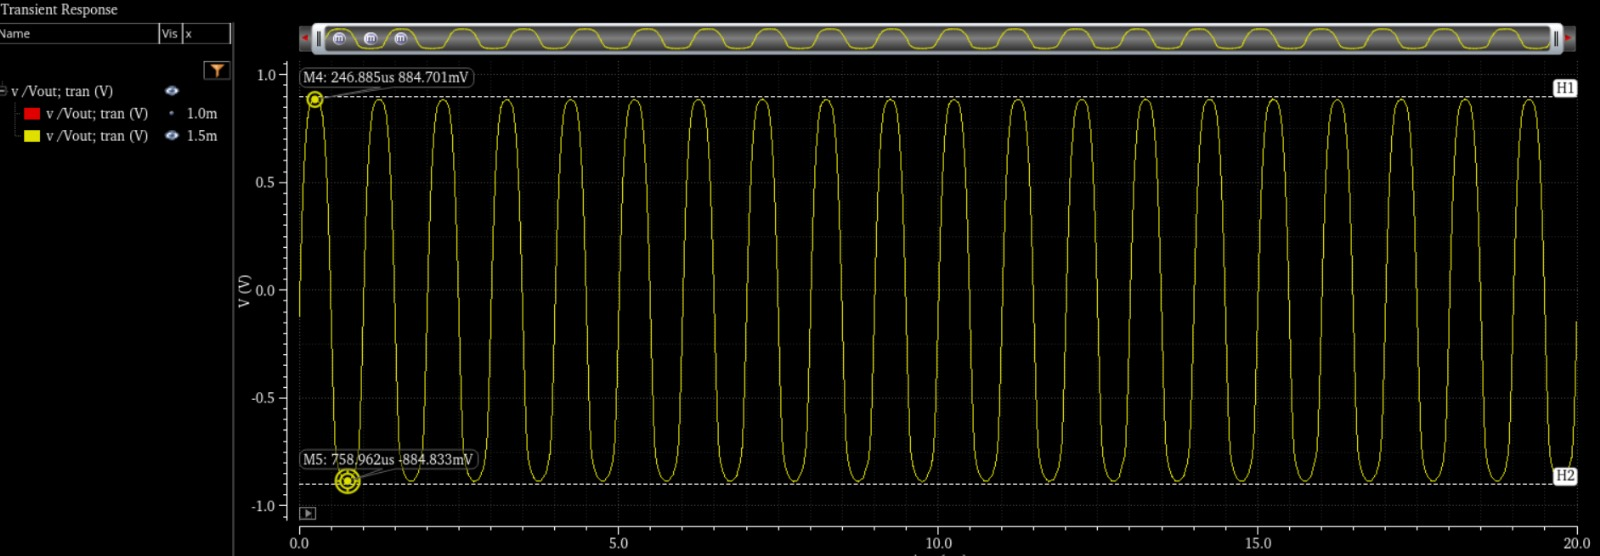
\includegraphics[width=0.7\textwidth]{swing.jpg}
    \caption{Measured output swing of the CMOS OTA.}
    \label{fig:swing}
\end{figure}


% Graphs
\section*{Figures}
\begin{figure}[H]
    \centering
    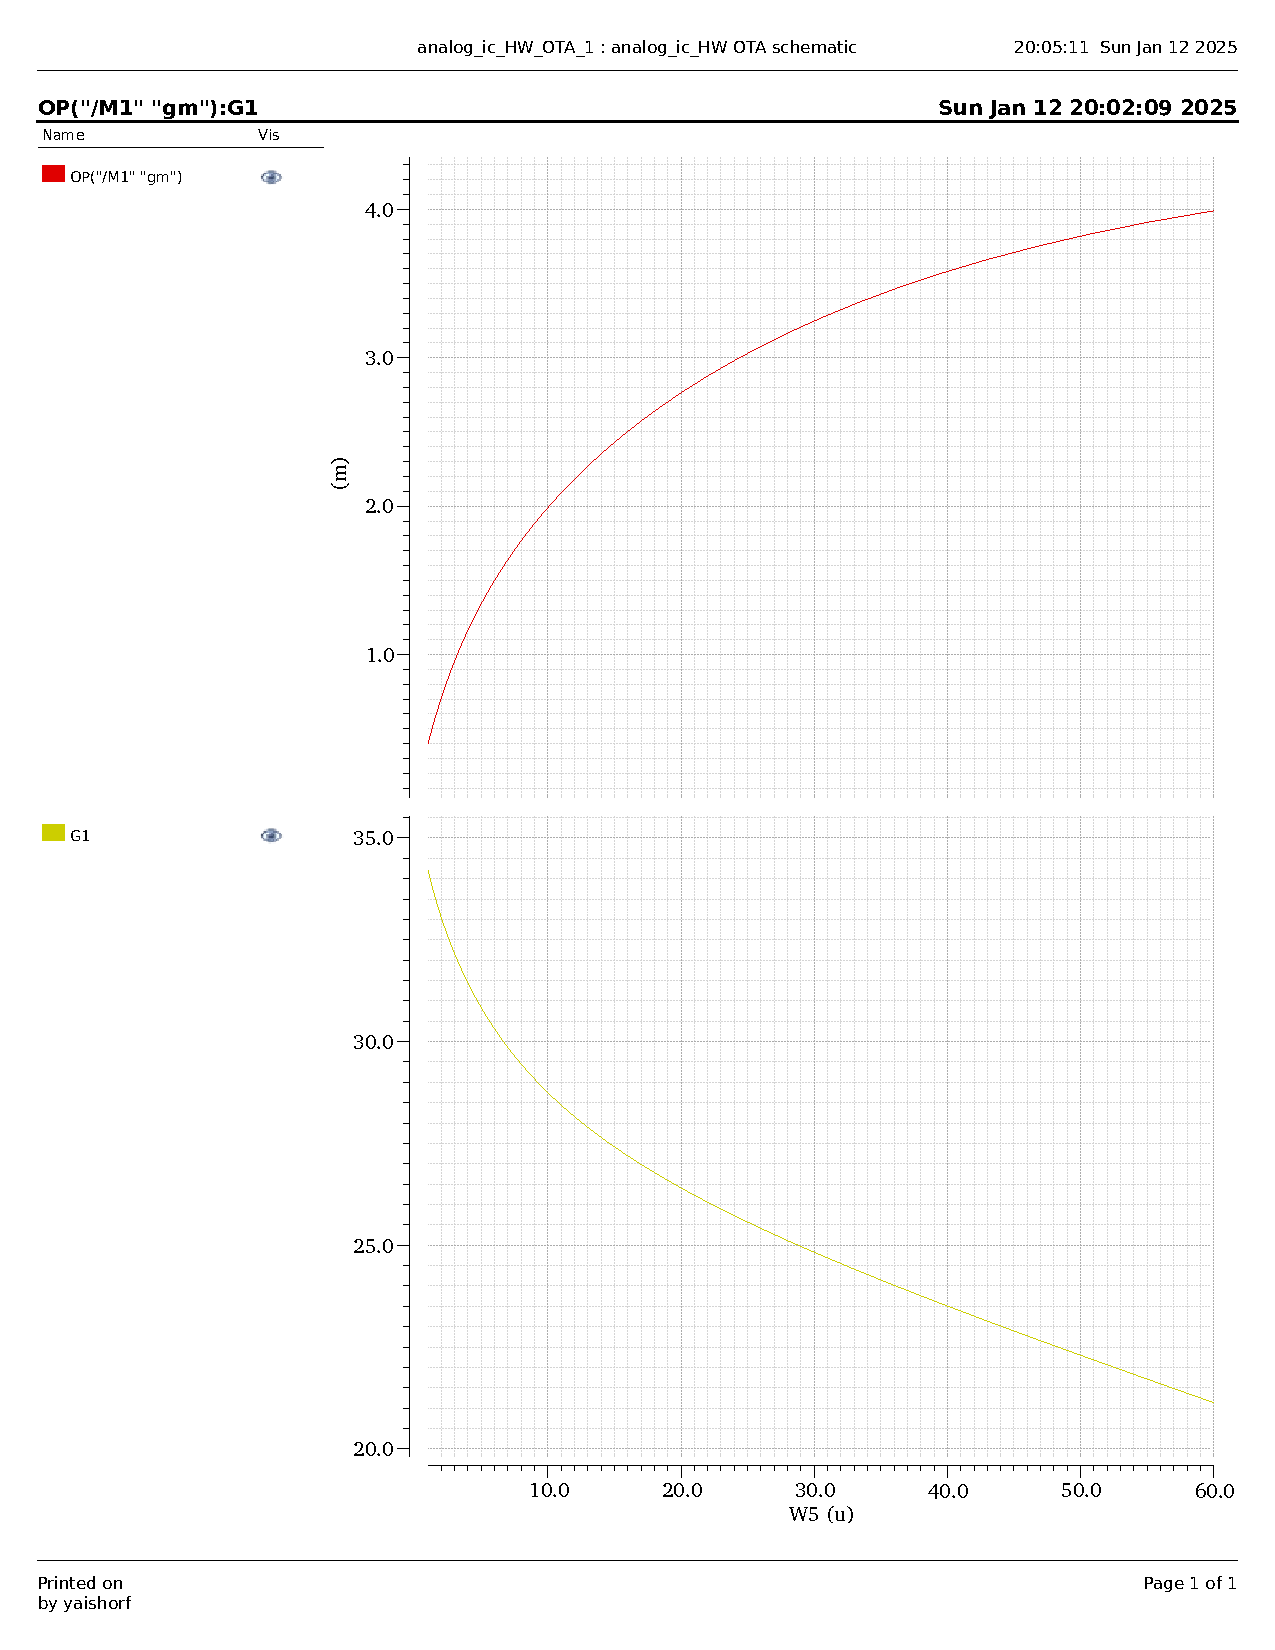
\includegraphics[width=0.8\textwidth]{gm1_W5.pdf}
    \caption{The impact of $W_5$ on $g_{m1}$ and stage gain.}
    \label{fig:gm1_w5}
\end{figure}

\begin{figure}[H]
    \centering
    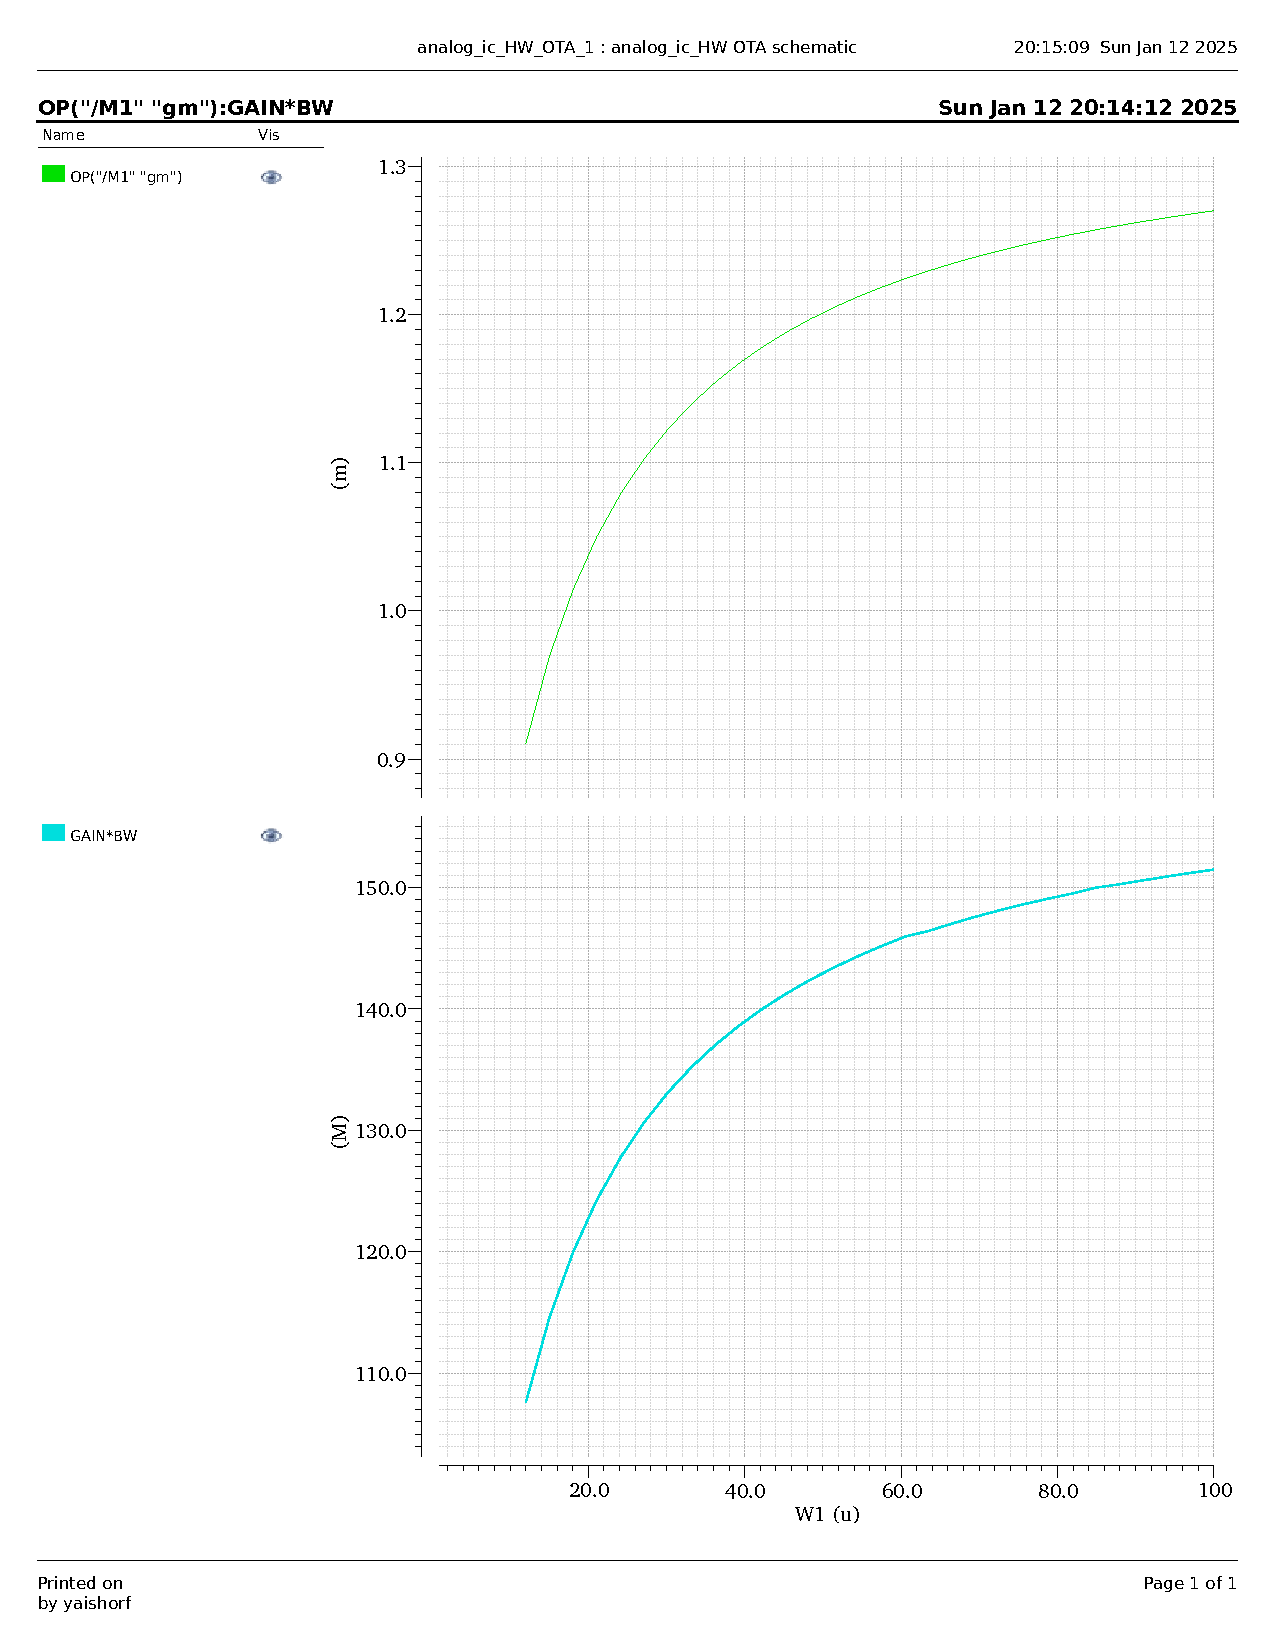
\includegraphics[width=0.8\textwidth]{gm1_W1.pdf}
    \caption{The relationship between $g_{m1}$ and GBW as a function of $W_1$.}
    \label{fig:gm1_w1}
\end{figure}

\begin{figure}[H]
    \centering
    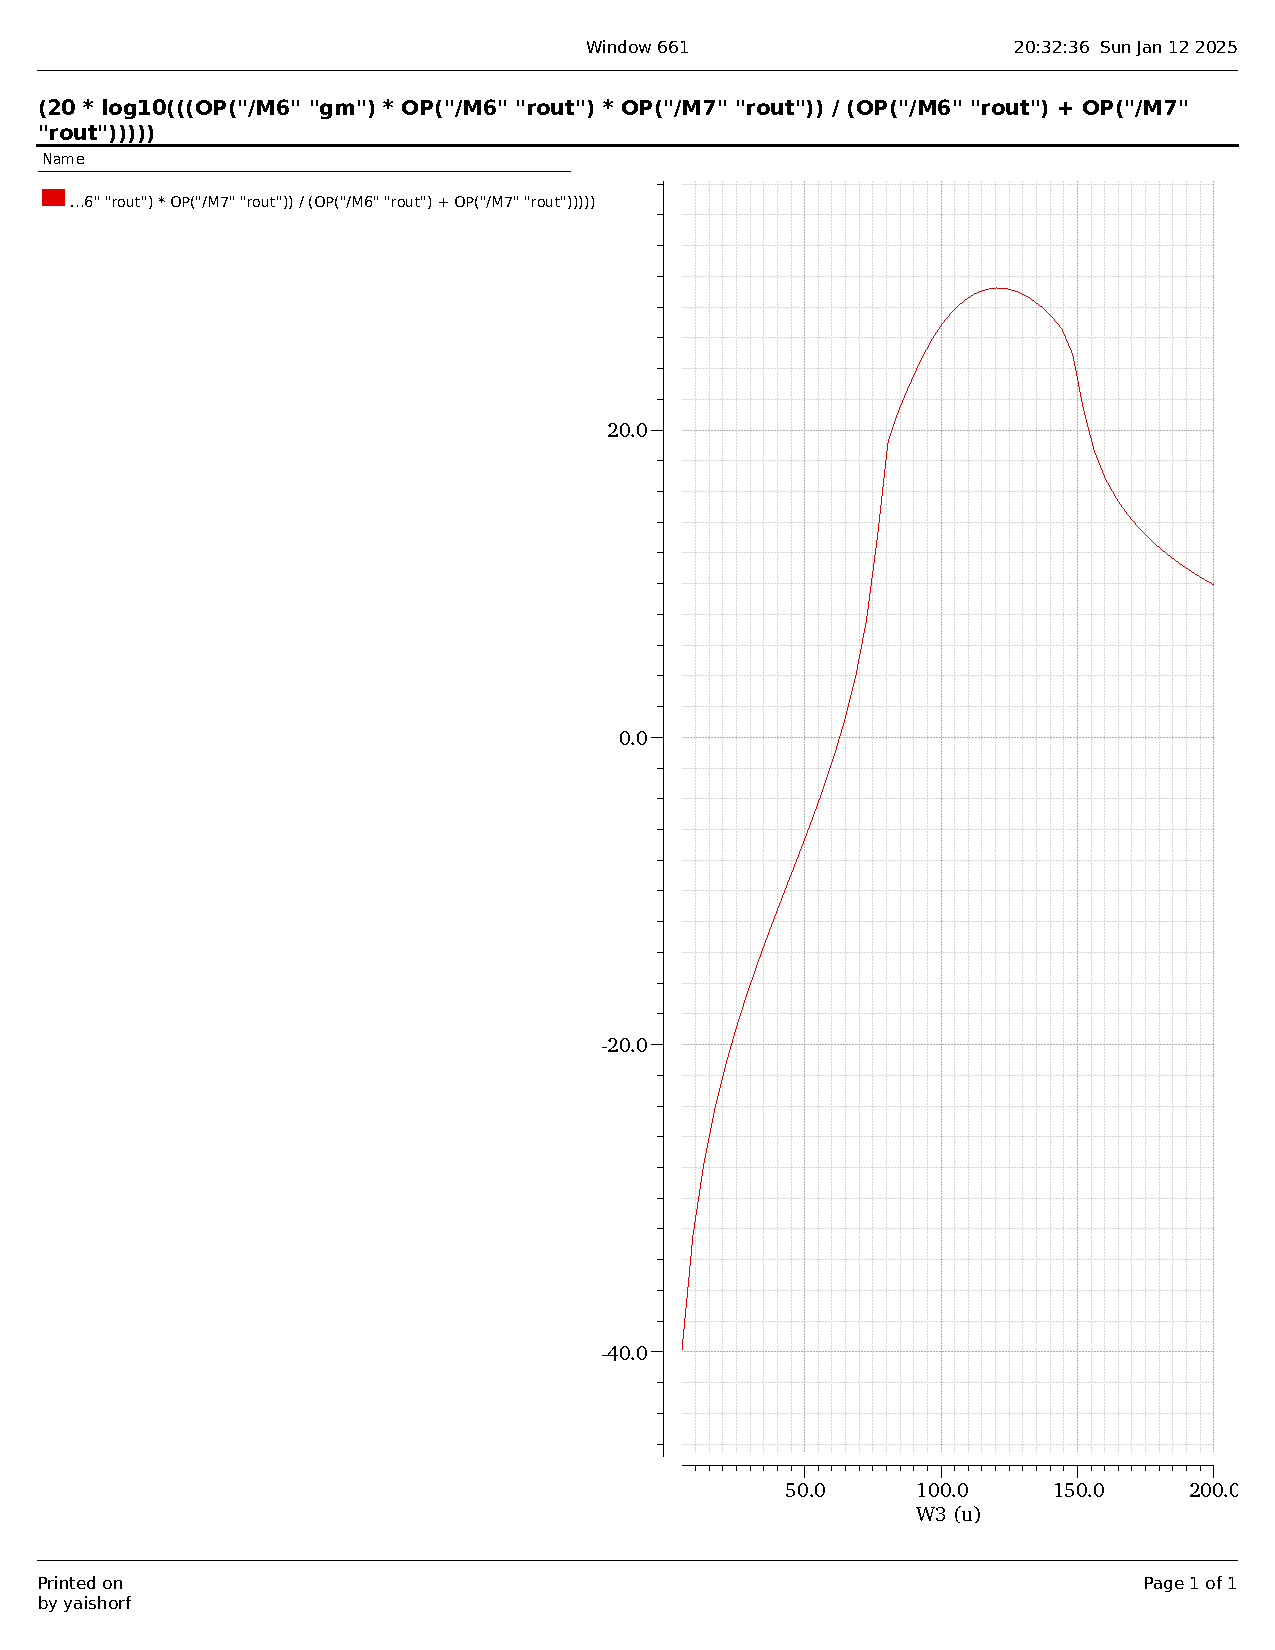
\includegraphics[width=0.8\textwidth]{G2_W4.pdf}
    \caption{The gain of the second stage versus $W_4$.}
    \label{fig:G2_W4}
\end{figure}

\begin{figure}[H]
    \centering
    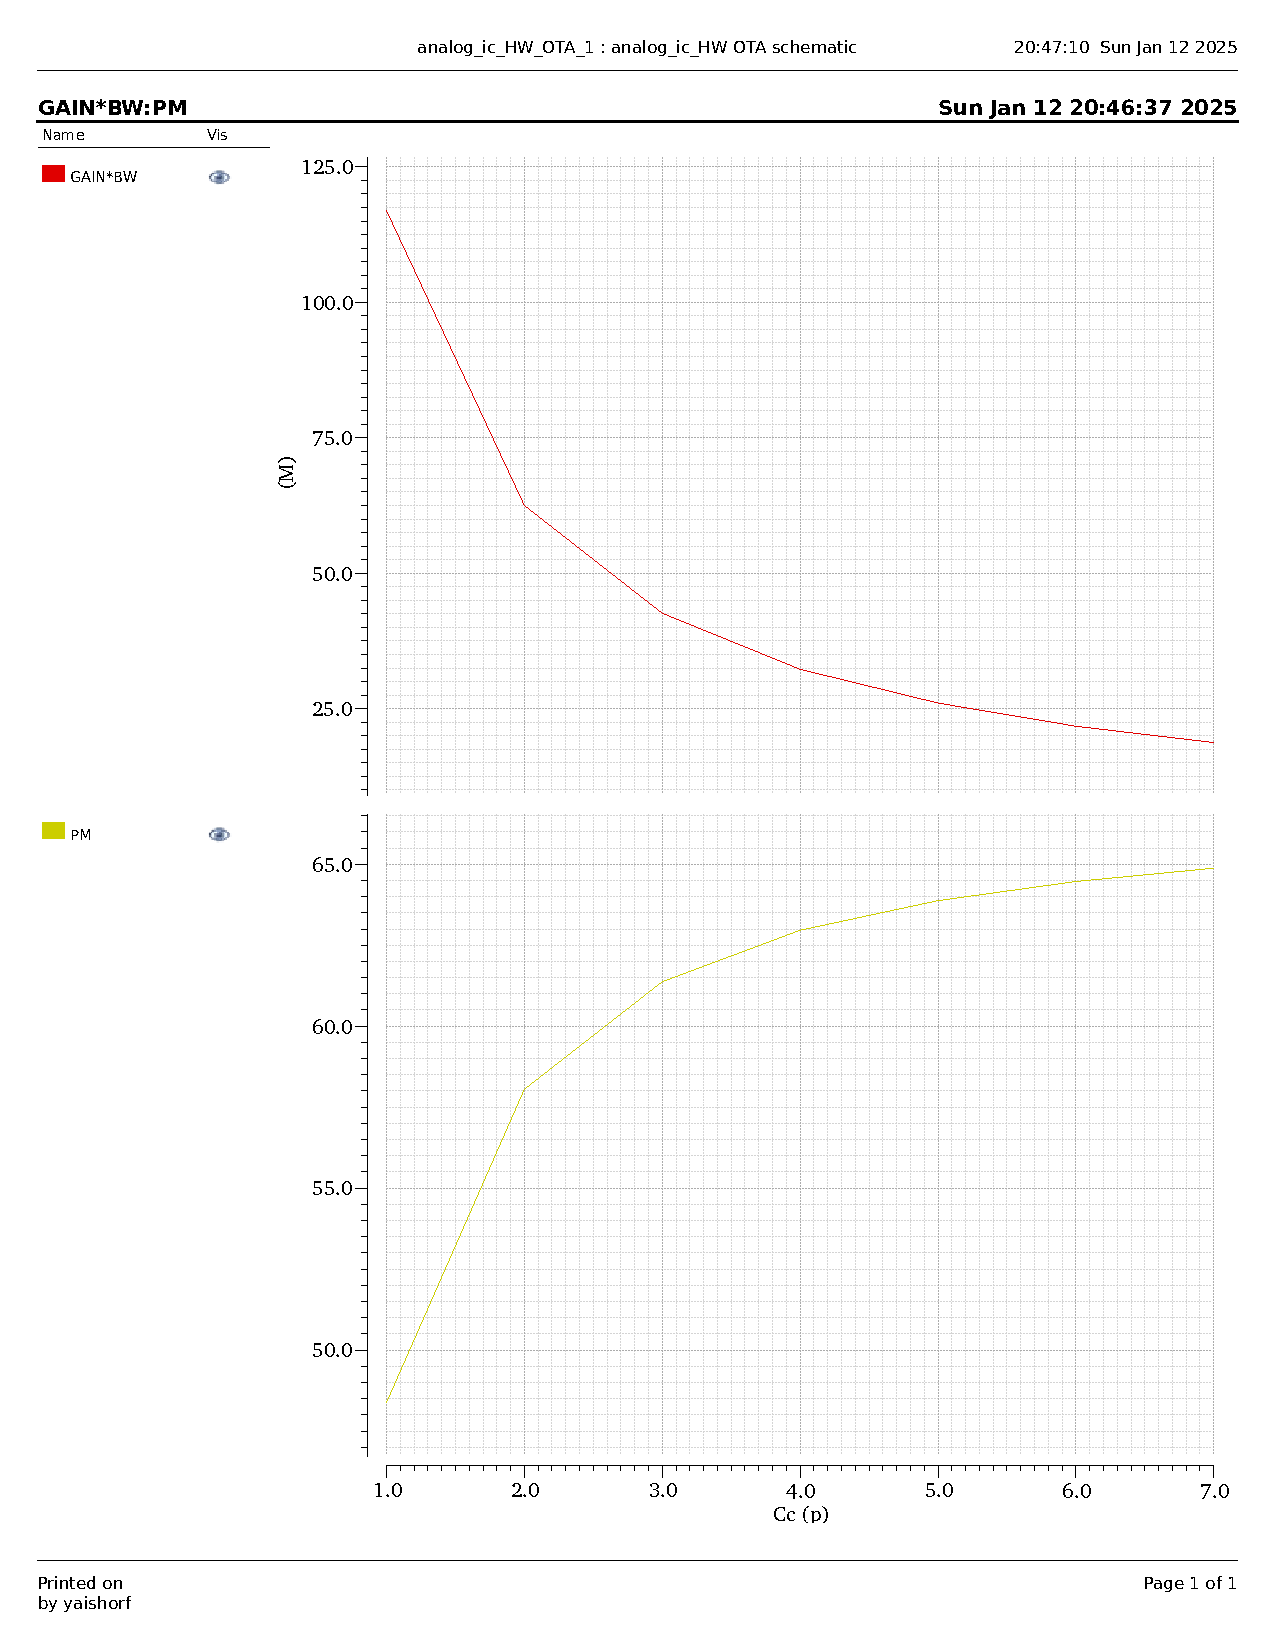
\includegraphics[width=0.8\textwidth]{GBW_Cc.pdf}
    \caption{GBW and PM as functions of $C_c$.}
    \label{fig:GBW_Cc}
\end{figure}

\begin{figure}[H]
    \centering
    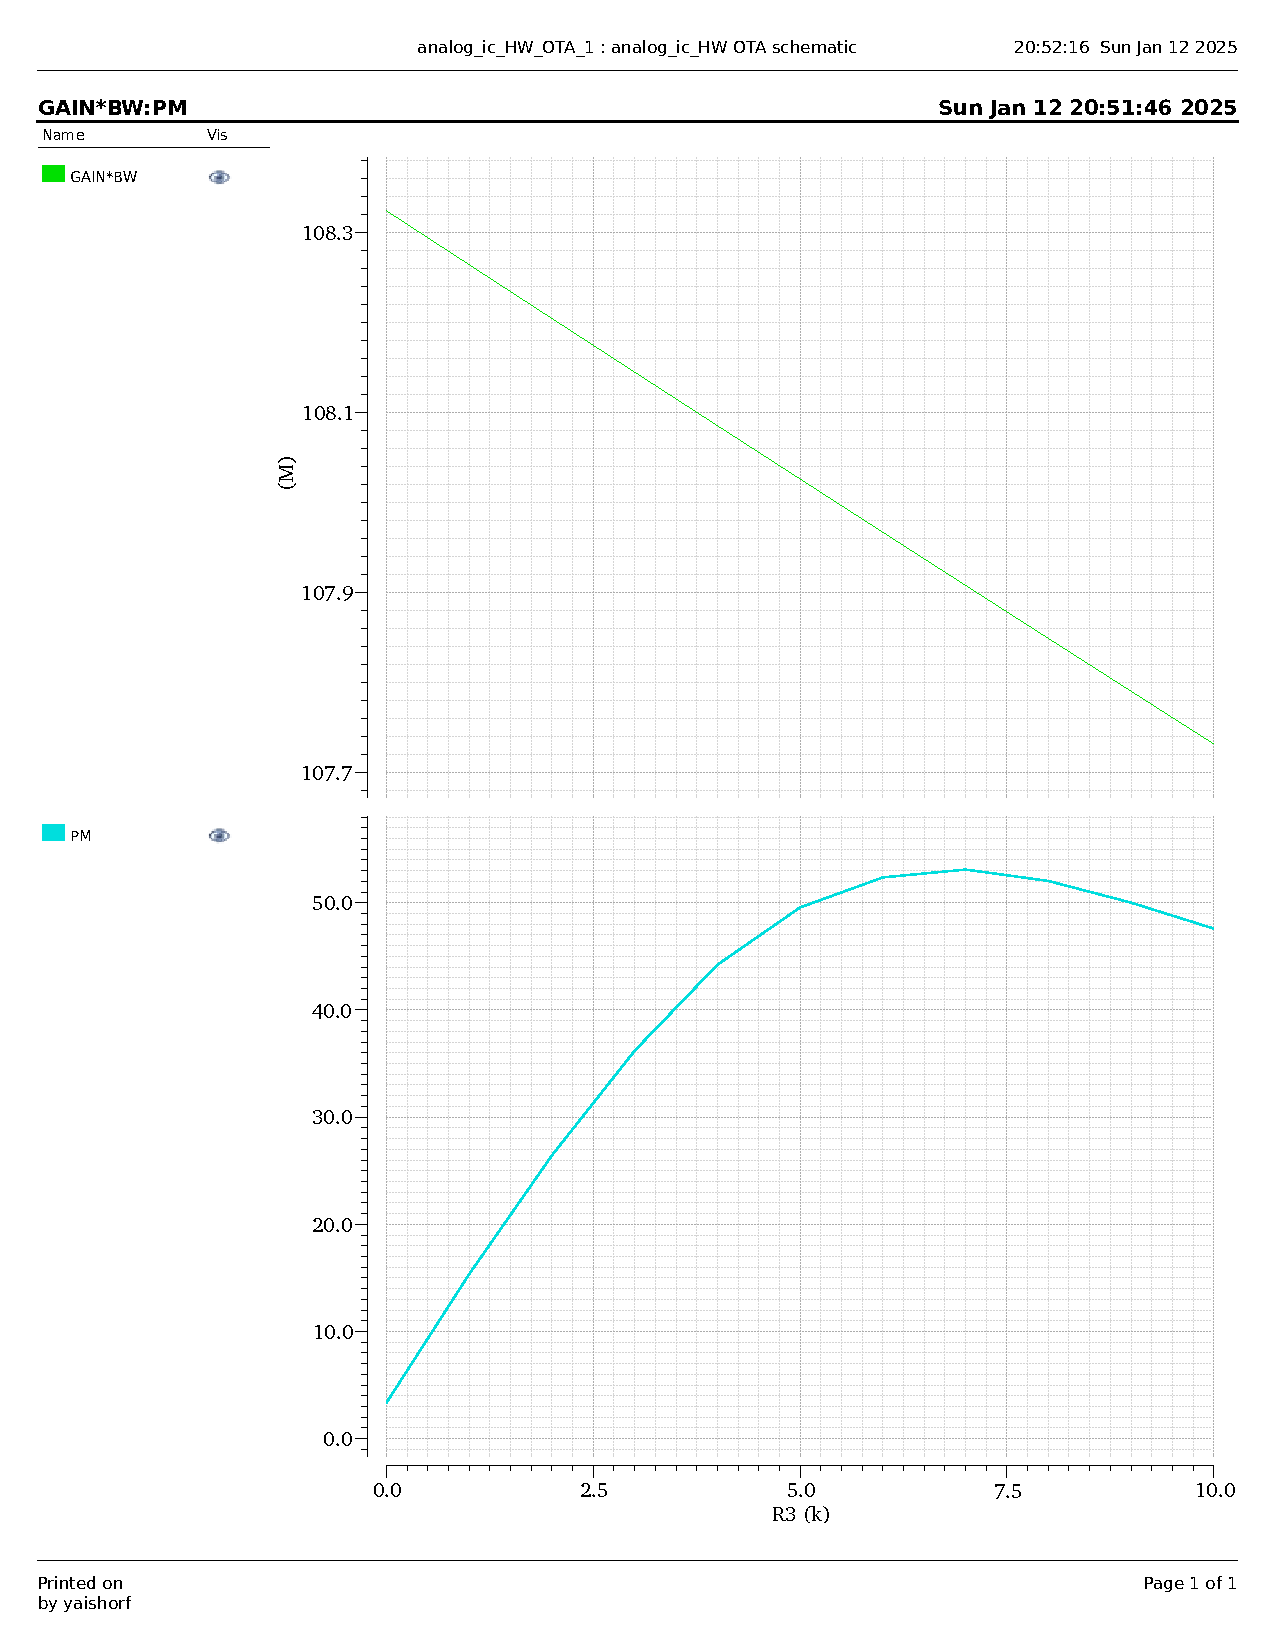
\includegraphics[width=0.8\textwidth]{GBW_R3.pdf}
    \caption{Effect of $R_3$ on GBW and PM.}
    \label{fig:GBW_R3}
\end{figure}



\end{document}